% !TEX root = thesis.tex

\section{Results}
\label{sec:exp}

\subsection{statistics}
Number of jets in different datasets and with different jet finders is shown in table \ref{tab:stats}. Background statistics for number of background cones (number of jets minus number of discarded cones) are shown in table \ref{tab:bgstats}. Ratio of background cones to number of jets is shown in table \ref{tab:bgratio}. The likelihood of having to discard a jet from background calculation is about 1-2\%.
\begin{table}[h]
\caption{Number of found jets by dataset and jet $p_T$ bin}
\tiny
\begin{tabular}{c | c | c | c | c | c | c | c | c | c}
Jet $p_T$   &     5-10 & 10-20  & 20-30 & 30-40 & 40-60 & 60-80 & 80-100 & 100-150 & 150-500 \\
MBFullR04 & 4969393 & 621753 & 32552 & 5584 & 1974 & 310 & 90 & 37 & 5 \\
MBFullR05 & 4750567 & 826598 & 42373 & 5543 & 1719 & 276 & 73 & 29 & 3 \\
MBChargedR04 & 3144538 & 673419 & 37783 & 4121 & 1009 & 148 & 36 & 12 & 1 \\
MBChargedR05 & 2229247 & 175763 & 7961 & 1270 & 410 & 61 & 12 & 3 \\
TriggeredFullR04 & 187557 & 115927 & 78138 & 51317 & 39262 & 8621 & 2409 & 1167 & 171 \\
TriggeredFullR05 & 99991 & 77147 & 48612 & 34325 & 28104 & 6342 & 1726 & 794 & 104 \\
TriggeredChargedR04 & 37411 & 29945 & 18186 & 13148 & 11142 & 2517 & 675 & 326 & 44 \\
TriggeredChargedR05 & 433155 & 175031 & 54789 & 19776 & 10626 & 1983 & 457 & 194 & 15 \\
\end{tabular}
\label{tab:stats}
\end{table}

\begin{table}[h]
\caption{Number of background cones used in perpendicular cone background calculation}
\label{tab:bgstats}
\tiny
\begin{tabular}{c | c | c | c | c | c | c | c | c | c}
Jet $p_T$     &   5-10 & 10-20  & 20-30 & 30-40 & 40-60 & 60-80 & 80-100 & 100-150 & 150-500 \\
MBFullR04 & 4947583 & 617895 & 32357 & 5548 & 1965 & 310 & 90 & 37 & 5 \\
MBFullR05 & 4710217 & 815461 & 41584 & 5439 & 1698 & 273 & 73 & 29 & 3 \\
MBChargedR04 & 3117495 & 661106 & 36739 & 4014 & 988 & 144 & 36 & 12 & 1 \\
MBChargedR05 & 2195286 & 172919 & 7860 & 1249 & 406 & 61 & 12 & 3 \\
TriggeredFullR04 & 186574 & 115376 & 77949 & 51216 & 39196 & 8603 & 2405 & 1167 & 171 \\
TriggeredFullR05 & 99102 & 76462 & 48320 & 34216 & 28038 & 6334 & 1722 & 794 & 103 \\
TriggeredChargedR04 & 37160 & 29543 & 17988 & 13099 & 11129 & 2515 & 675 & 326 & 44 \\
TriggeredChargedR05 & 313421 & 140707 & 45229 & 16243 & 8709 & 1604 & 377 & 154 & 14 \\
\end{tabular}
\end{table}

\begin{table}[h]
\caption{Ratio of background cone number to number of jets}
\label{tab:bgratio}
\tiny
\begin{tabular}{c | c | c | c | c | c | c | c | c | c}
MBFullR04 & 99.56\% & 99.38\% & 99.40\% & 99.36\% & 99.54\% & 100.00\% & 100.00\% & 100.00\% & 100.00\% \\
MBFullR05 & 99.15\% & 98.65\% & 98.14\% & 98.12\% & 98.78\% & 98.91\% & 100.00\% & 100.00\% & 100.00\% \\
MBChargedR04 & 99.14\% & 98.17\% & 97.24\% & 97.40\% & 97.92\% & 97.30\% & 100.00\% & 100.00\% & 100.00\% \\
MBChargedR05 & 98.48\% & 98.38\% & 98.73\% & 98.35\% & 99.02\% & 100.00\% & 100.00\% & 100.00\% \\
TriggeredFullR04 & 99.48\% & 99.52\% & 99.76\% & 99.80\% & 99.83\% & 99.79\% & 99.83\% & 100.00\% & 100.00\% \\
TriggeredFullR05 & 99.11\% & 99.11\% & 99.40\% & 99.68\% & 99.77\% & 99.87\% & 99.77\% & 100.00\% & 99.04\% \\
TriggeredChargedR04 & 99.33\% & 98.66\% & 98.91\% & 99.63\% & 99.88\% & 99.92\% & 100.00\% & 100.00\% & 100.00\% \\
TriggeredChargedR05 & 72.36\% & 80.39\% & 82.55\% & 82.13\% & 81.96\% & 80.89\% & 82.49\% & 79.38\% & 93.33\% \\
\end{tabular}
\end{table}


\subsection{Data}
%\begin{figure}[htp]
%\centering
%%\begin{subfigure}{0.95\textwidth}
%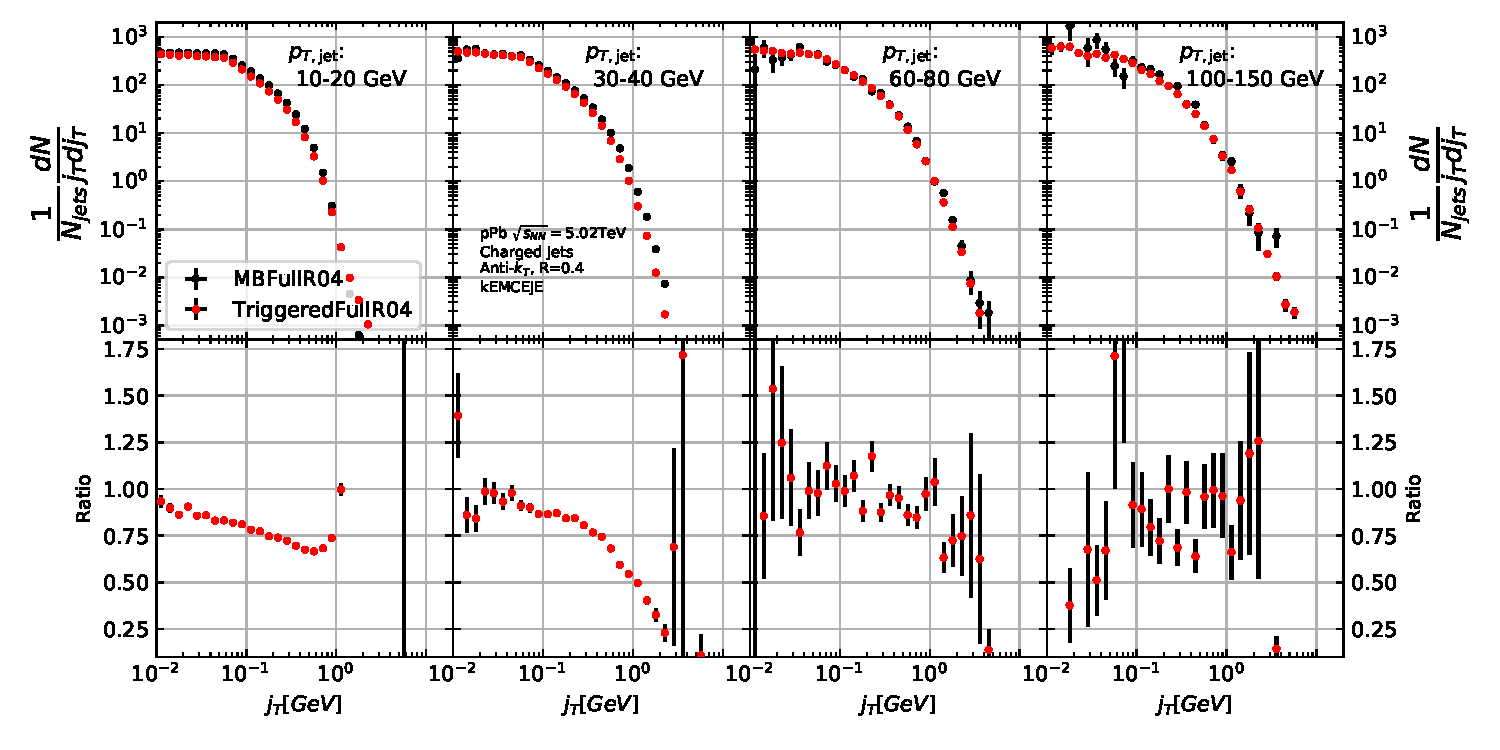
\includegraphics[width=0.95\textwidth]{results/MBvsTriggeredFullJetsR04JetConeJt.pdf} 
%%Tag 20170810 python2.7 Python/MBtoTriggeredComparison.py legotrain_CF_pPb-1053_20170223-2002_LHC13bcde.root
%
%%\includegraphics[width=0.95\textwidth]{results/OverlayjetjtIncl_T02_\figComment}
%\caption{Comparison between minimum bias and triggered datasets }
%%\end{subfigure}
%%\begin{subfigure}{0.5\textwidth}
%%%\includegraphics[width=0.95\textwidth]{results/OverlayjetjtIncl_T06_\figComment}
%%%\caption{Jet $p_T$ 80-100 GeV}
%%\end{subfigure}
%\end{figure}



\subsection{Background}
Comparison between perpendicular cone and random background in figure \ref{fig:bgcomparison}.
\begin{figure}
\centering
\begin{subfigure}{0.95\textwidth}
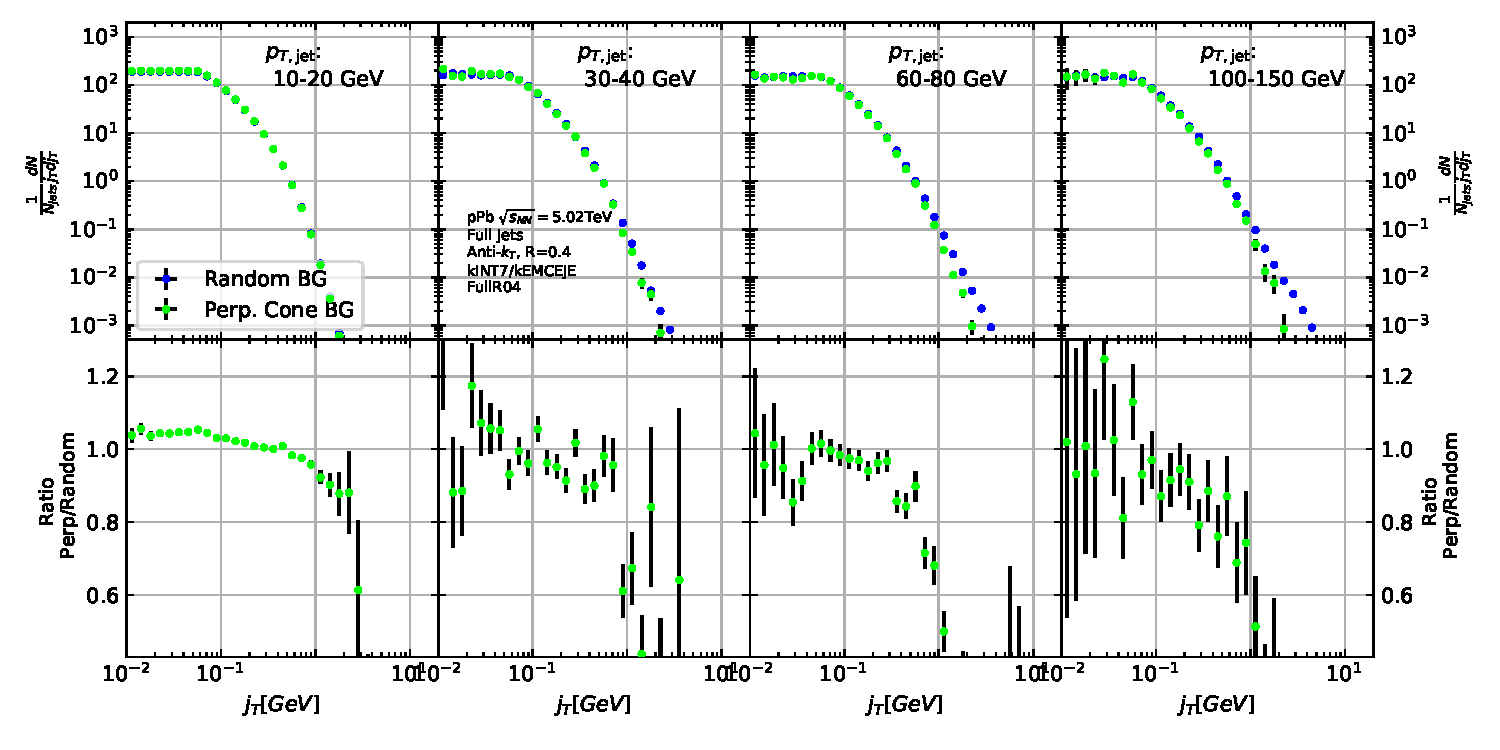
\includegraphics[width=\textwidth]{results/MixedFullJetsR04BackgroundComparison.pdf}
%Tag 20170810 python2.7 Python/InclusiveWithBackground.py legotrain_CF_pPb-1053_20170223-2002_LHC13bcde.root
\end{subfigure}
\caption{$j_T$ background with two different methods}
\label{fig:bgcomparison}
\end{figure}
%\subsubsection{Background problem}
%\begin{itemize}
%\item Certain cases have backgrounds larger than the inclusive
%\item Background $j_T$ in cone with radius R
%\item Inclusive $j_T$ for jet constituents from anti-$k_T$ algorithm with parameter $R$
%\item Part of the background already subtracted because of the algorithm?
%\end{itemize}

\subsection{Inclusive results}
Results in figure \ref{fig:inclusive}
\begin{figure}
\centering
\begin{subfigure}{0.95\textwidth}
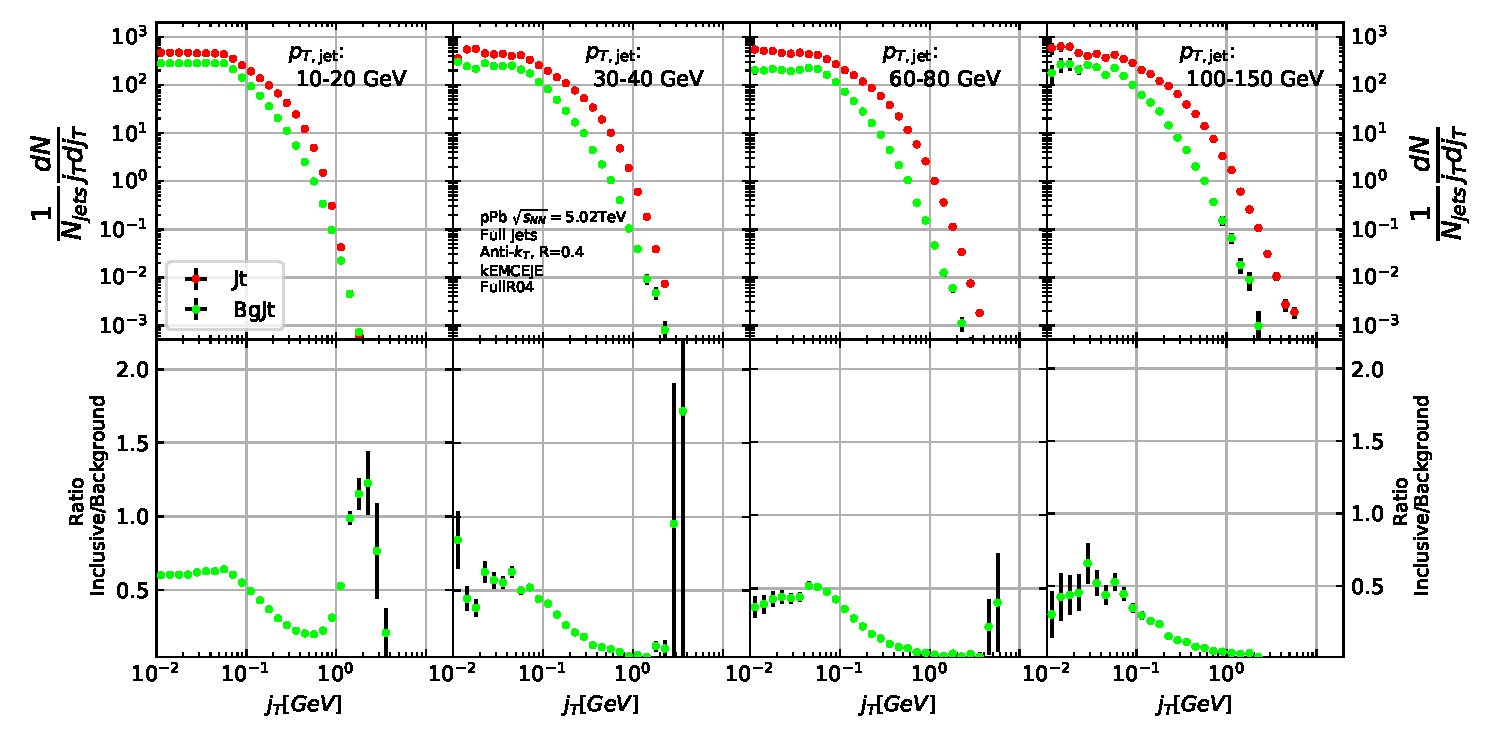
\includegraphics[width=\textwidth]{results/MixedFullJetsR04JetConeJtInclusive.pdf}
%Tag 20170810 python2.7 Python/InclusiveWithBackground.py legotrain_CF_pPb-1053_20170223-2002_LHC13bcde.root
\end{subfigure}
\caption{Inclusive $j_T$ with background}
\label{fig:inclusive}
\end{figure}

%\caption{Bad example}
%\end{subfigure}
%\begin{subfigure}{0.5\textwidth}
%\includegraphics[width=0.95\textwidth]{results/jetjtIncl_T06A04_\figComment}
%\caption{Good example}
%\end{subfigure}
%\end{figure}


\subsection{Comparison between A and C side}
In 2013 there were some issues with tracking. To rule out effects on $\jt{}$ distributions a study was performed comparing $j_T$ distributions between A and C side. No systematic differences were observed.

\begin{figure}
\centering
\begin{subfigure}{0.95\textwidth}
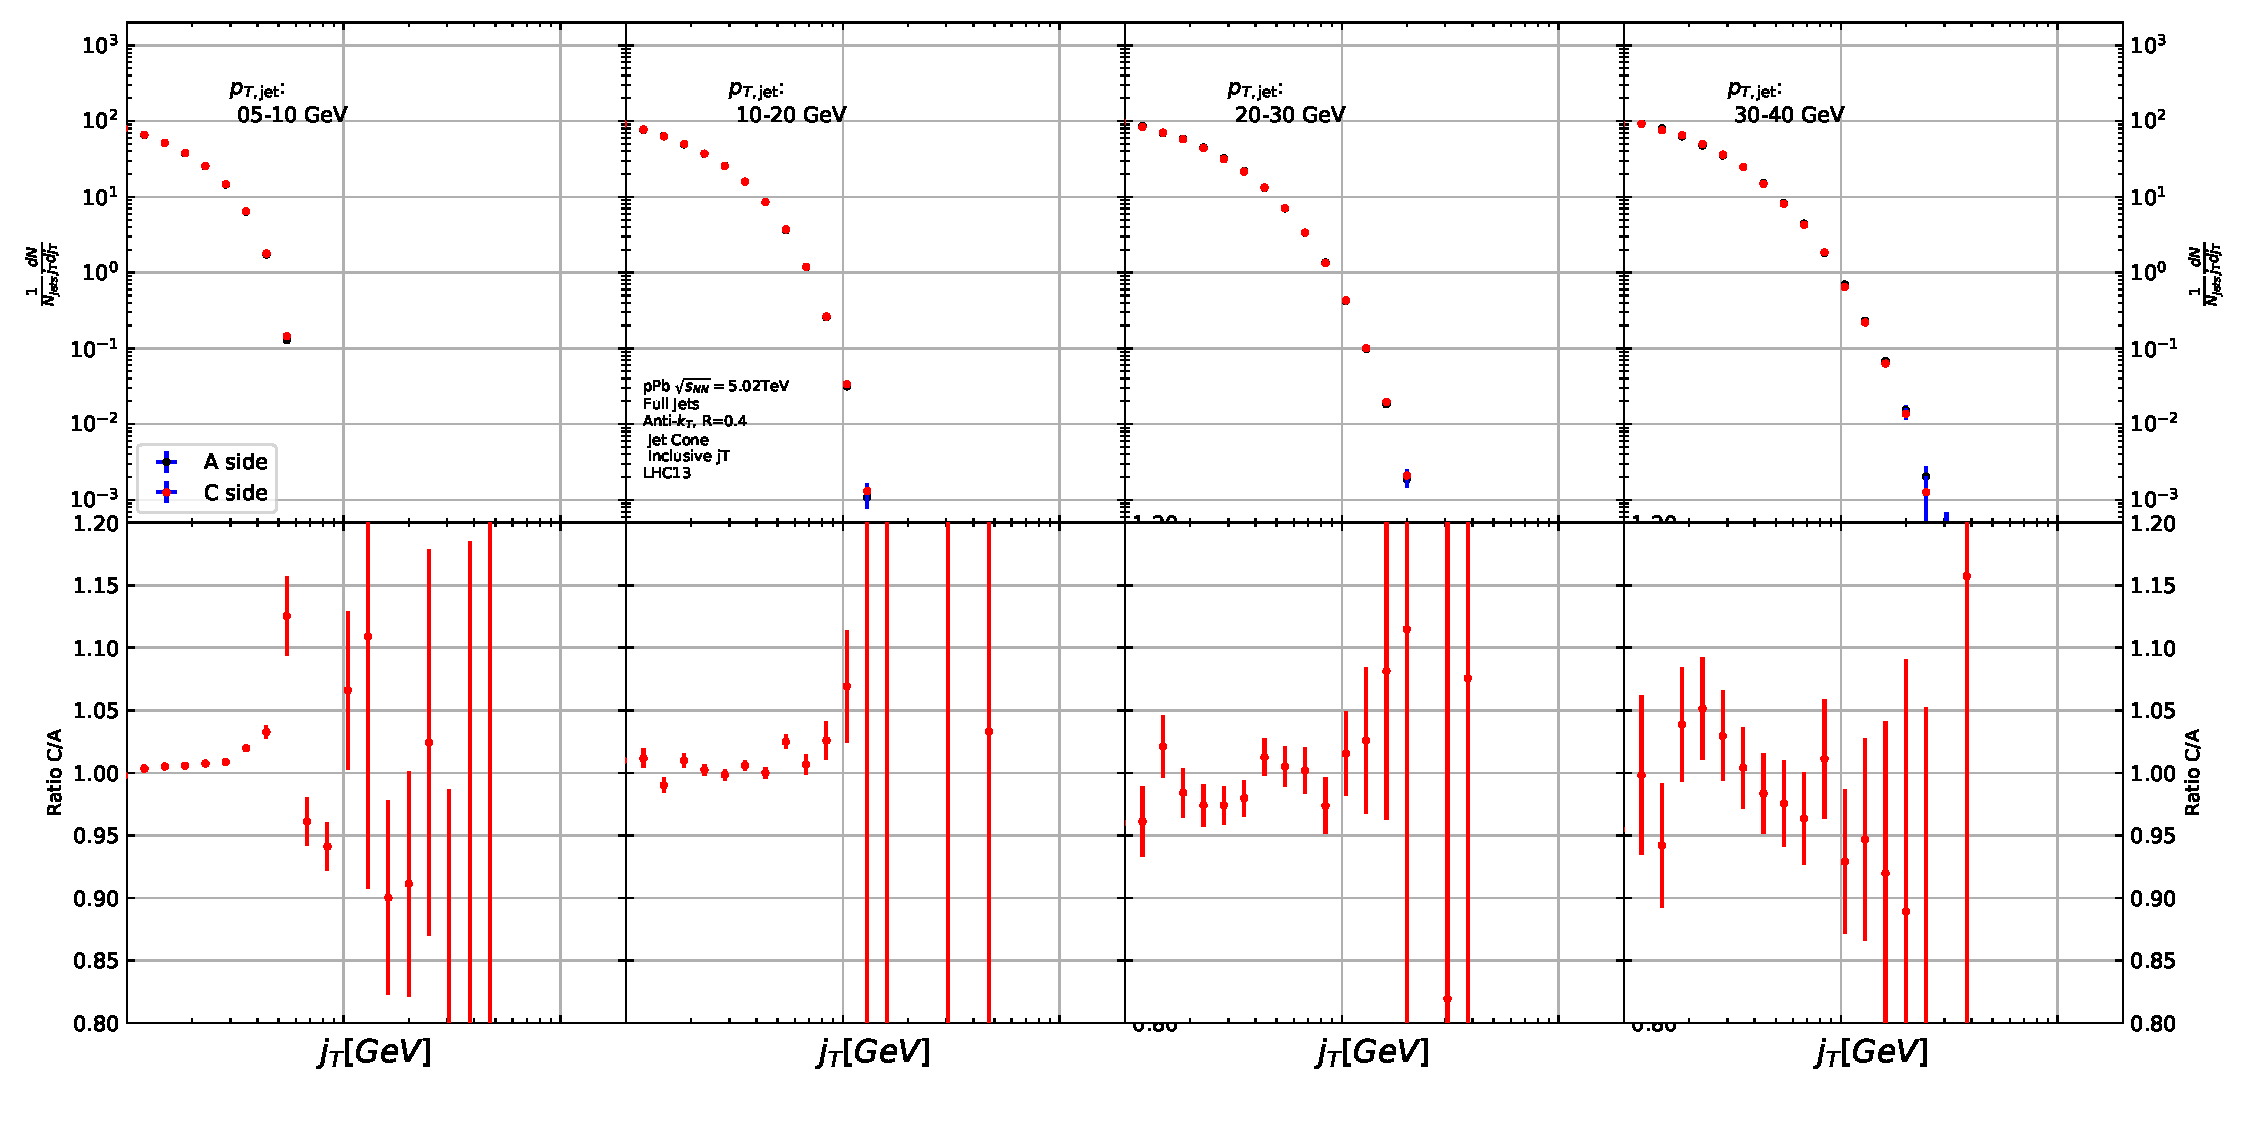
\includegraphics[width=\textwidth]{pics/ACsideComparison/ACsideJetConeJtInclusivePtFrom0To4LHC13.pdf}
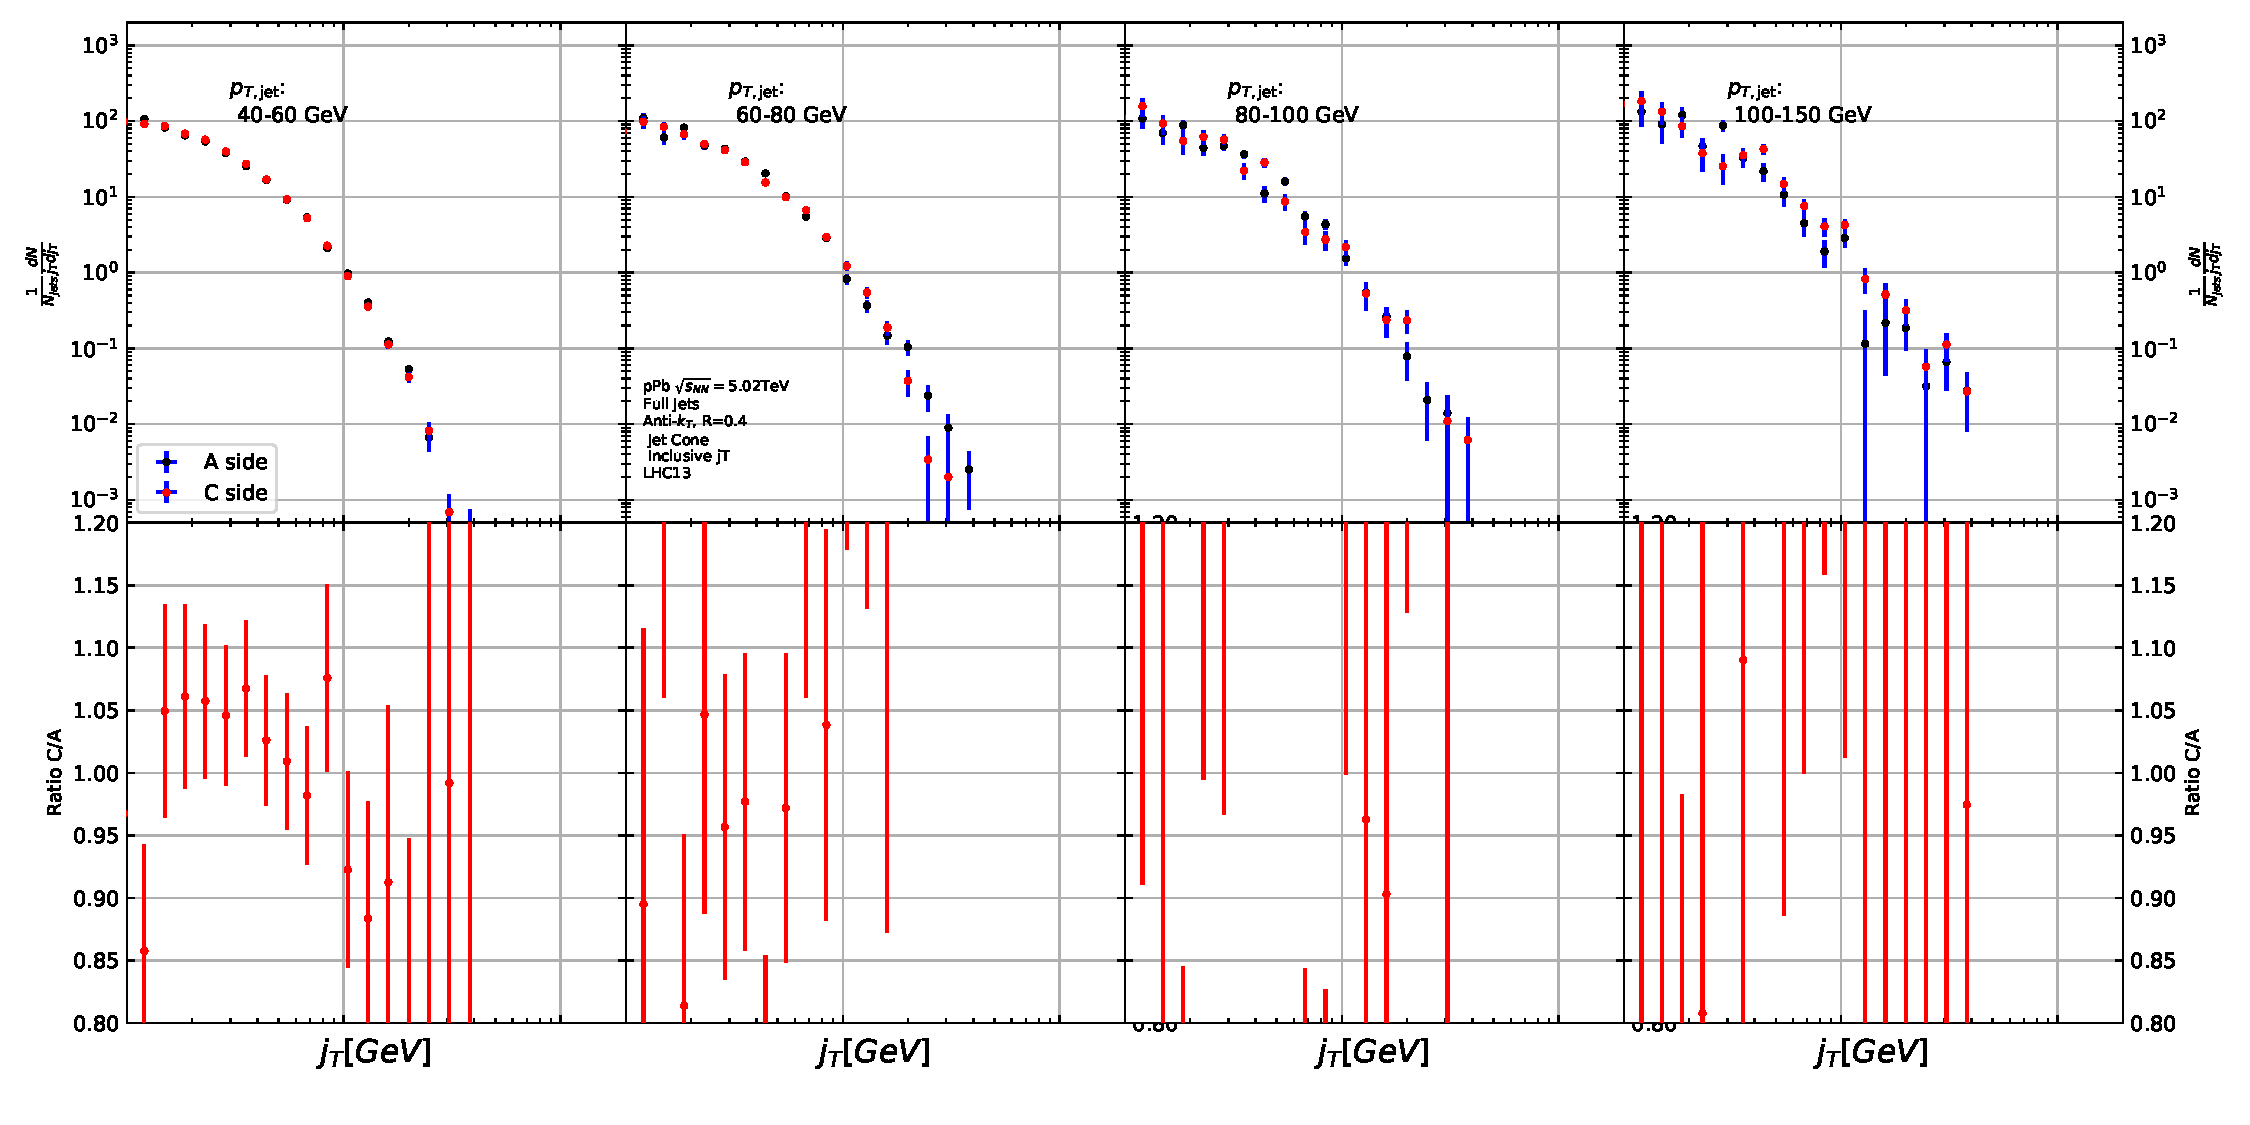
\includegraphics[width=\textwidth]{pics/ACsideComparison/ACsideJetConeJtInclusivePtFrom4To8LHC13.pdf}
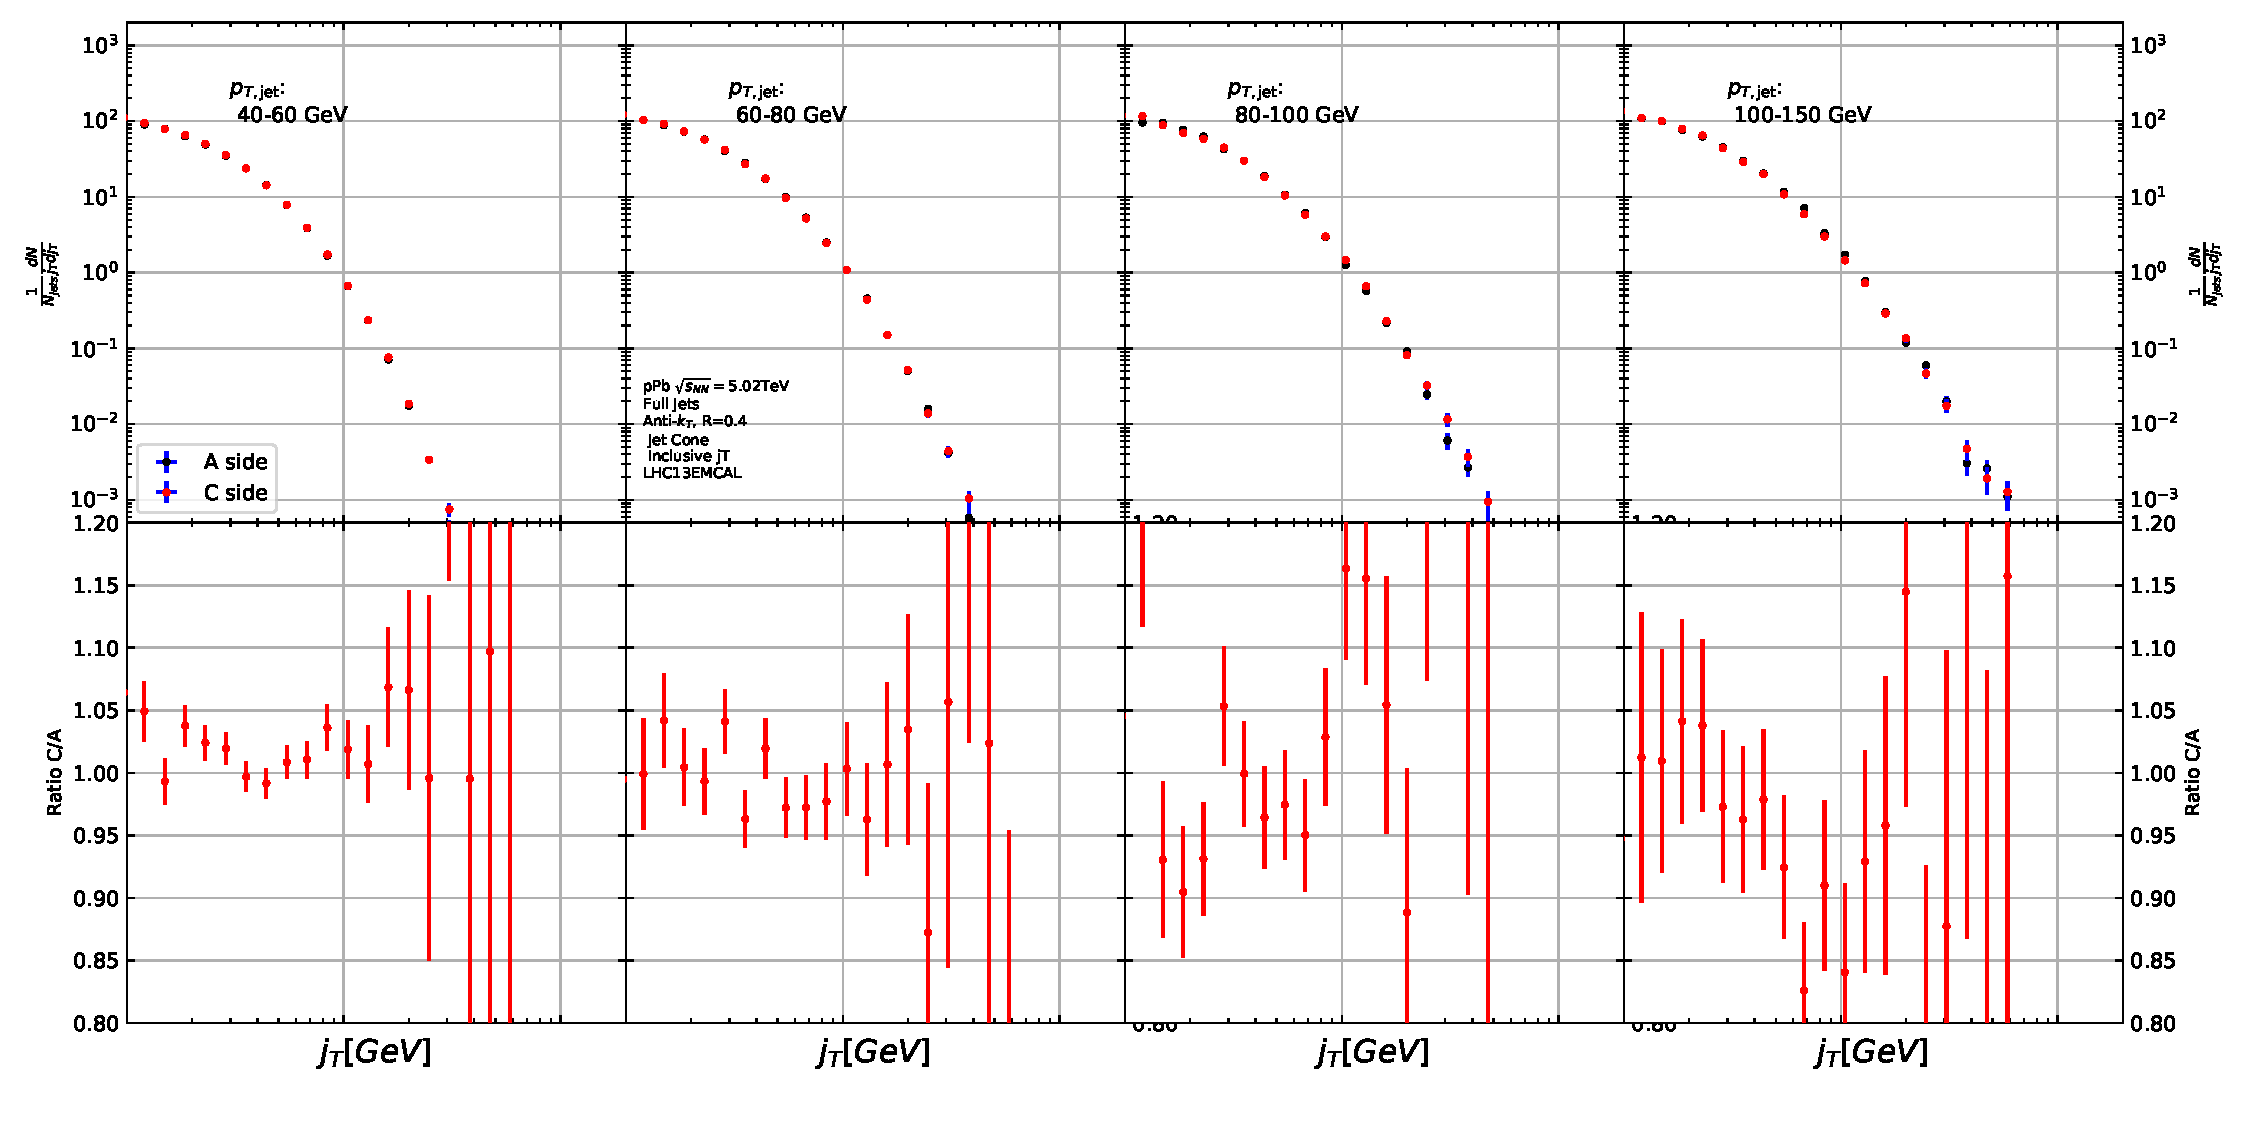
\includegraphics[width=\textwidth]{pics/ACsideComparison/ACsideJetConeJtInclusivePtFrom4To8LHC13EMCAL.pdf}
%Tag 20170810 python2.7 Python/DrawSignal.py legotrain_CF_pPb-1053_20170223-2002_LHC13bcde.root
\end{subfigure}
\caption{Comparison of inclusive $j_T$ distributions between A and C side for minimum bias and EMCAL triggered data.}
\label{fig:signalbg}
\end{figure}

\subsection{Subtracted signal}
Results in figure \ref{fig:signal}. Comparison between signals with different backgrounds in figure \ref{fig:signalbg}
\begin{figure}
\centering
\begin{subfigure}{0.95\textwidth}
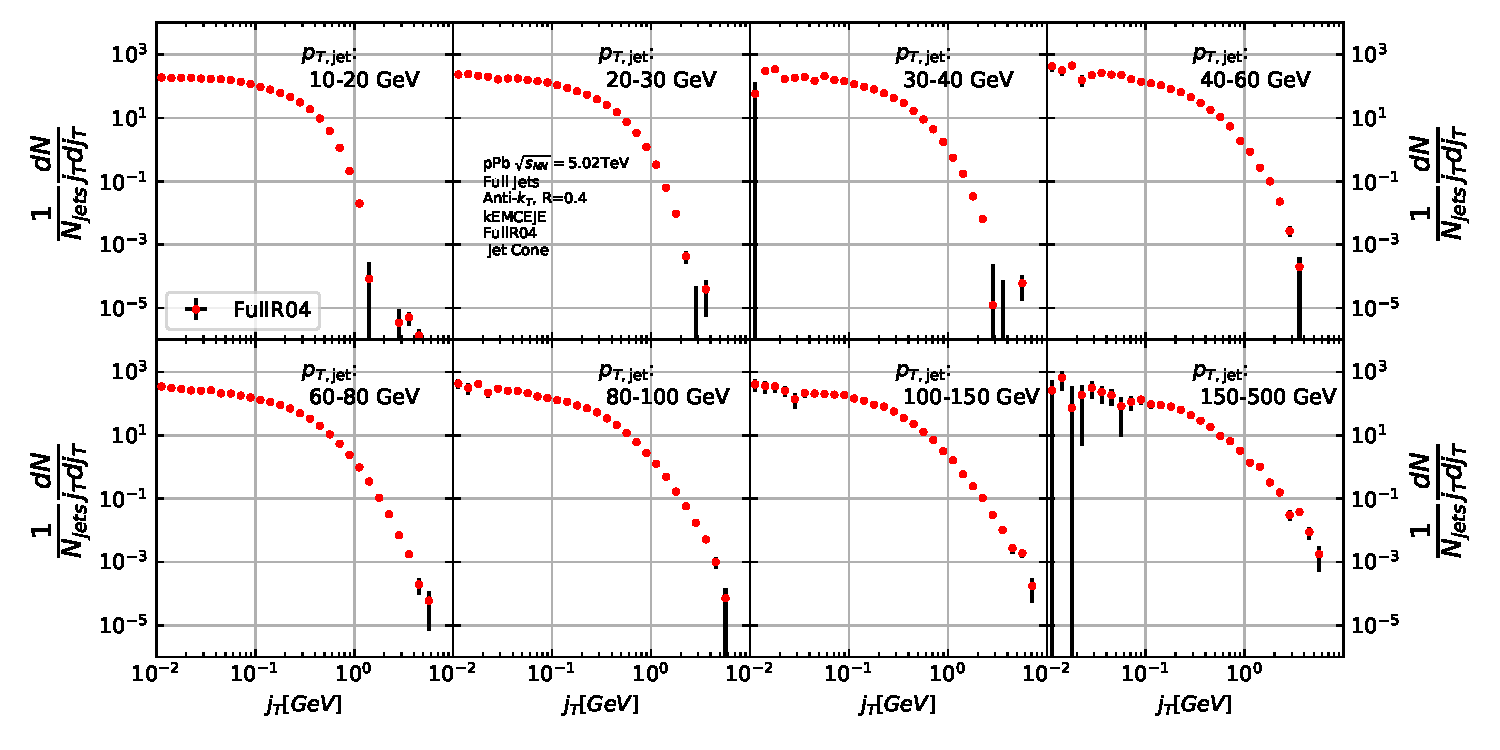
\includegraphics[width=\textwidth]{results/MixedFullJetsR04JetConeJtSignal.pdf}
%Tag 20170810 python2.7 Python/DrawSignal.py legotrain_CF_pPb-1053_20170223-2002_LHC13bcde.root
\end{subfigure}
\caption{$j_T$ signal with background subtracted}
\label{fig:signal}
\end{figure}

\begin{figure}
\centering
\begin{subfigure}{0.95\textwidth}
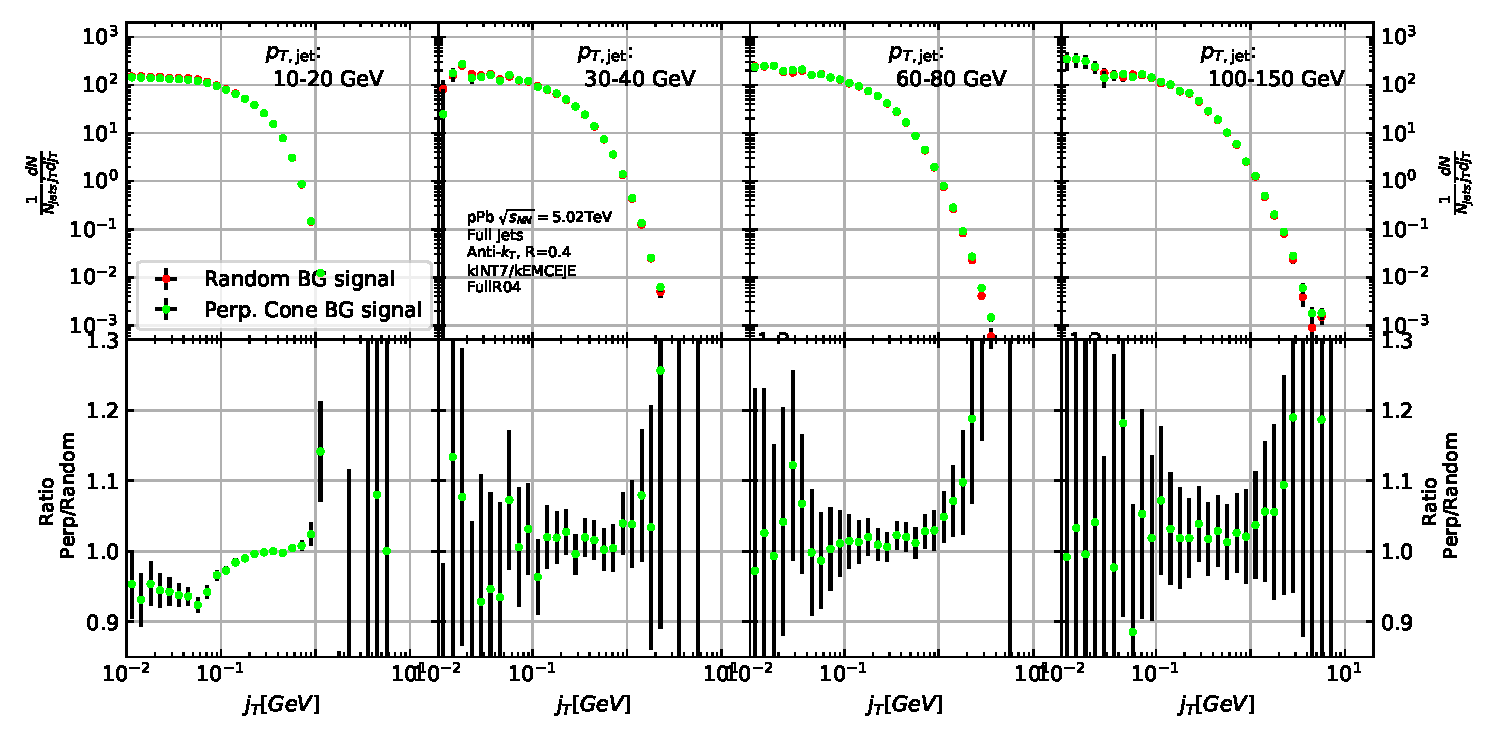
\includegraphics[width=\textwidth]{results/MixedFullJetsR04SignalBackgroundComparison.pdf}
%Tag 20170810 python2.7 Python/DrawSignal.py legotrain_CF_pPb-1053_20170223-2002_LHC13bcde.root
\end{subfigure}
\caption{Comparison of the effect of background method on $j_T$ signal.}
\label{fig:signalbg}
\end{figure}

\subsection{Fitting}
Fits of $j_T$ distributions in different jet $p_T$ bins with $p_T  > 40 \gev$ are shown in figure \ref{fig:fits}. Additional jet $p_T$ bins are shown in appendix \ref{app:a}. In lowest jet $p_T$ bins the jets are mainly combinatorial which makes background subtraction and unfolding difficult and thus the signal can't be trusted. 

The fits describe the data well. There is some fluctuation of the order of 10 \% around the fit function. At hight $j_T$ the statistical errors in the signal are large.

\begin{figure}
\centering
%\begin{subfigure}{0.24\textwidth}
%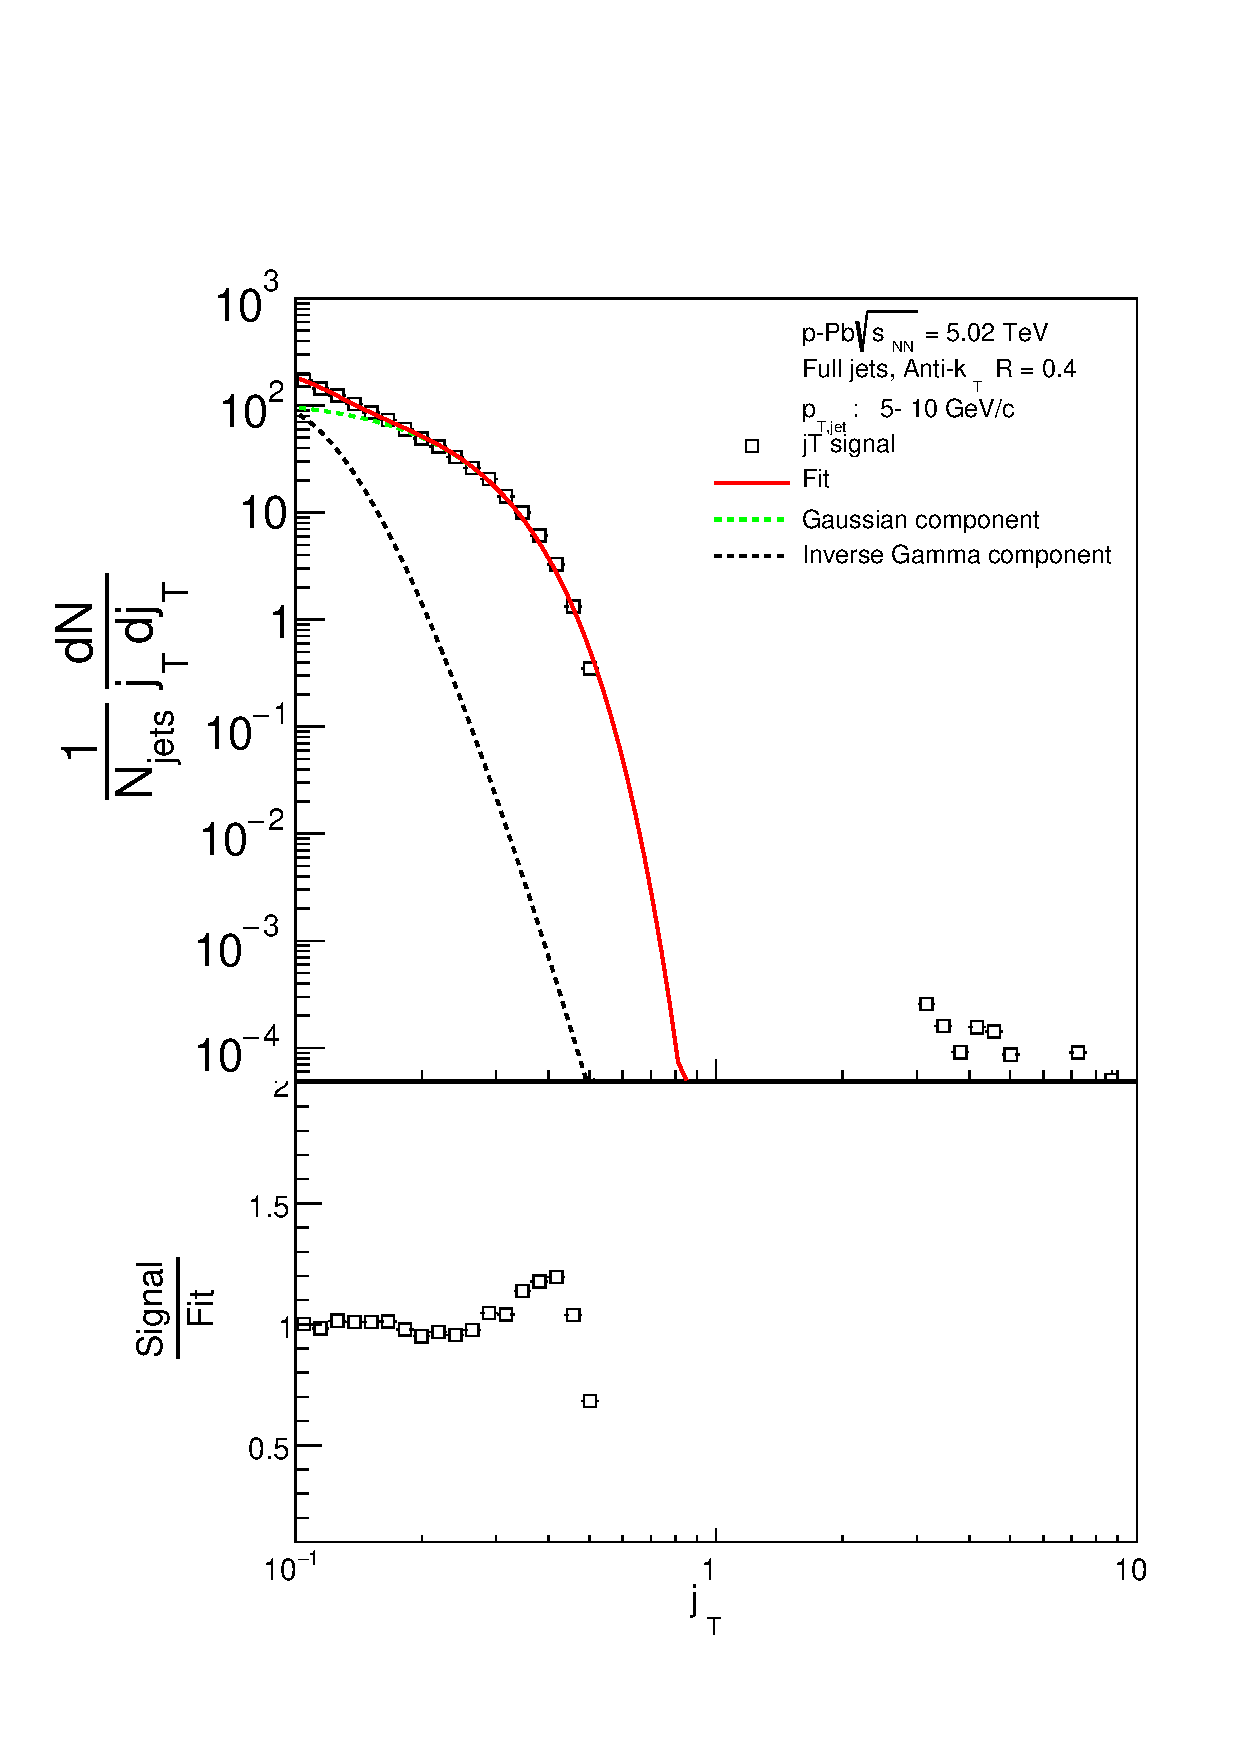
\includegraphics[width=0.95\textwidth]{RooUnfold/figs/JetConejTSignalFit/JetConejTSignalFitNFin00JetPt00perconeBgBayes}
%\end{subfigure}
%\begin{subfigure}{0.24\textwidth}
%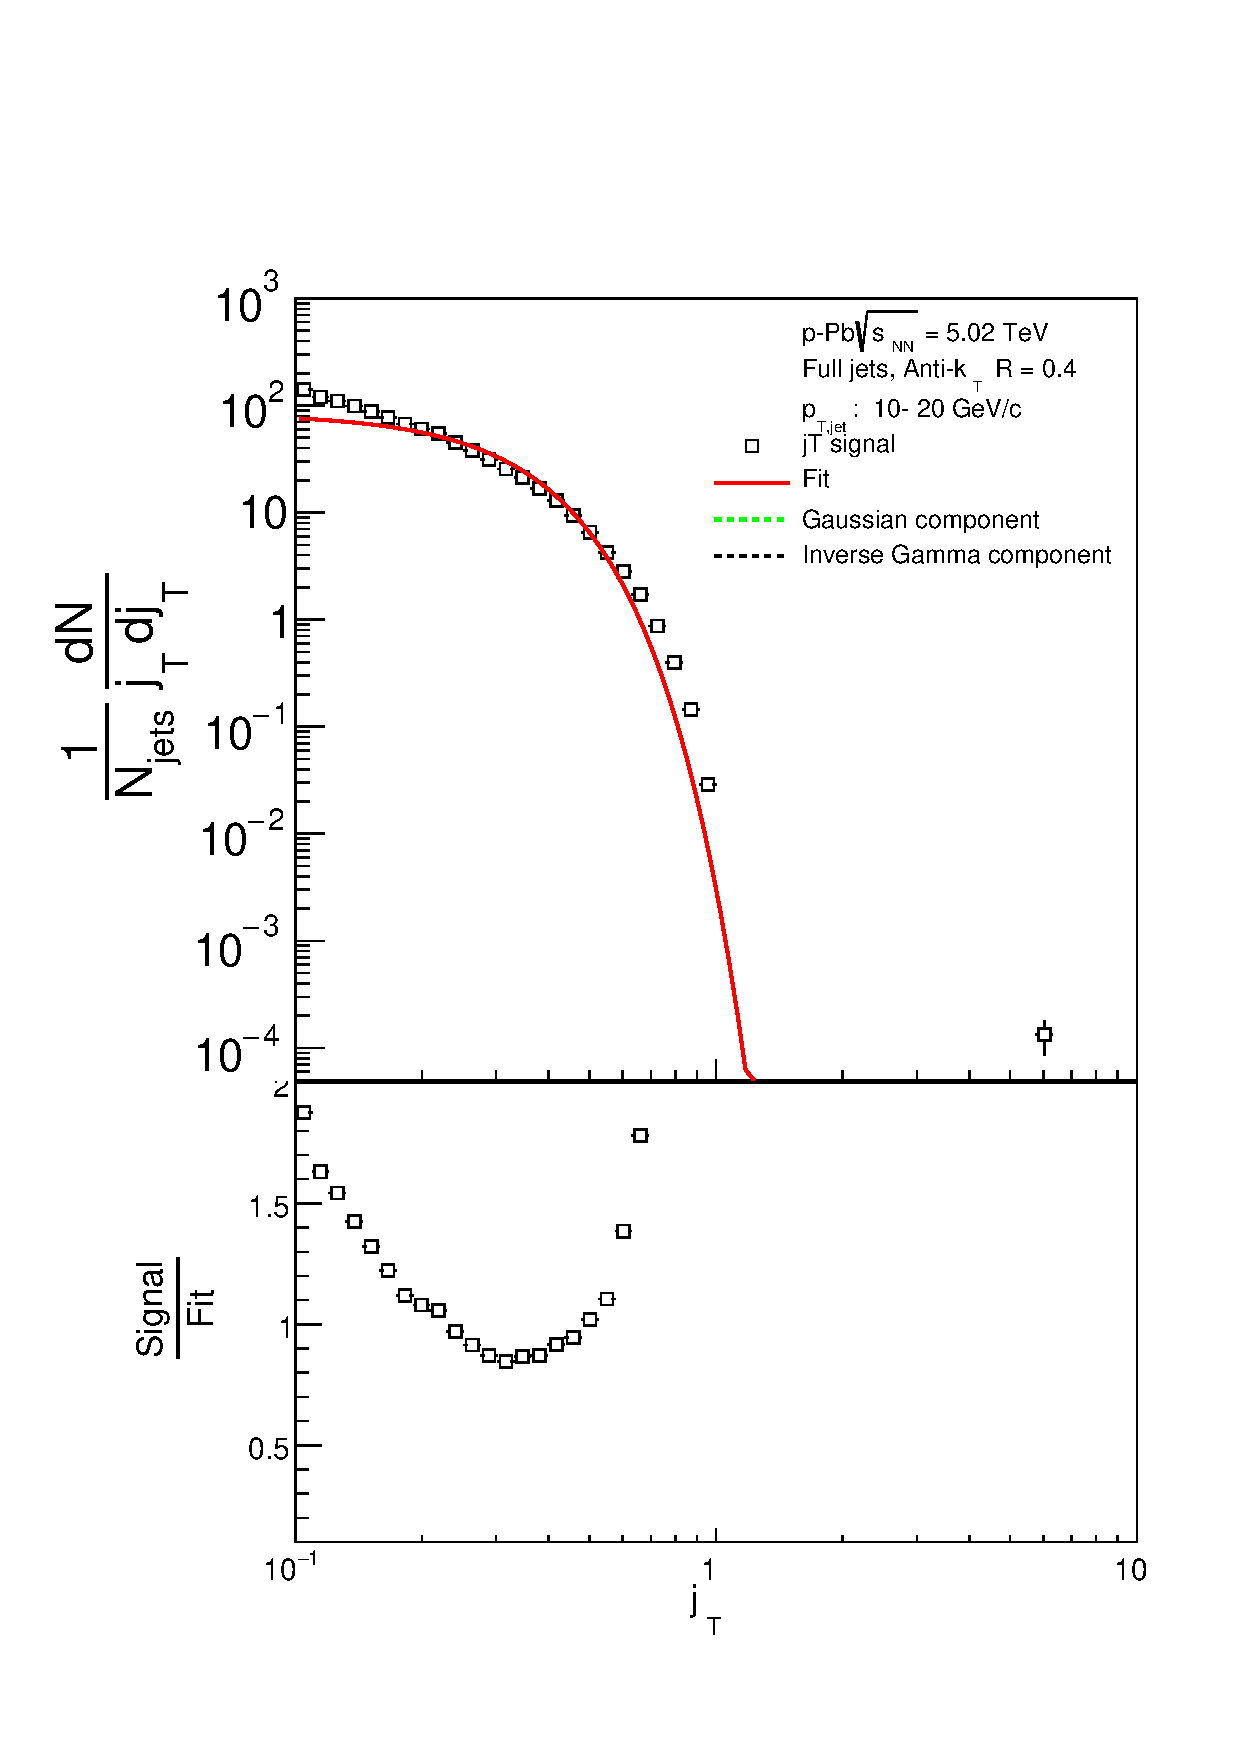
\includegraphics[width=0.95\textwidth]{RooUnfold/figs/JetConejTSignalFit/JetConejTSignalFitNFin00JetPt01perconeBgBayes}
%\end{subfigure}
%\begin{subfigure}{0.24\textwidth}
%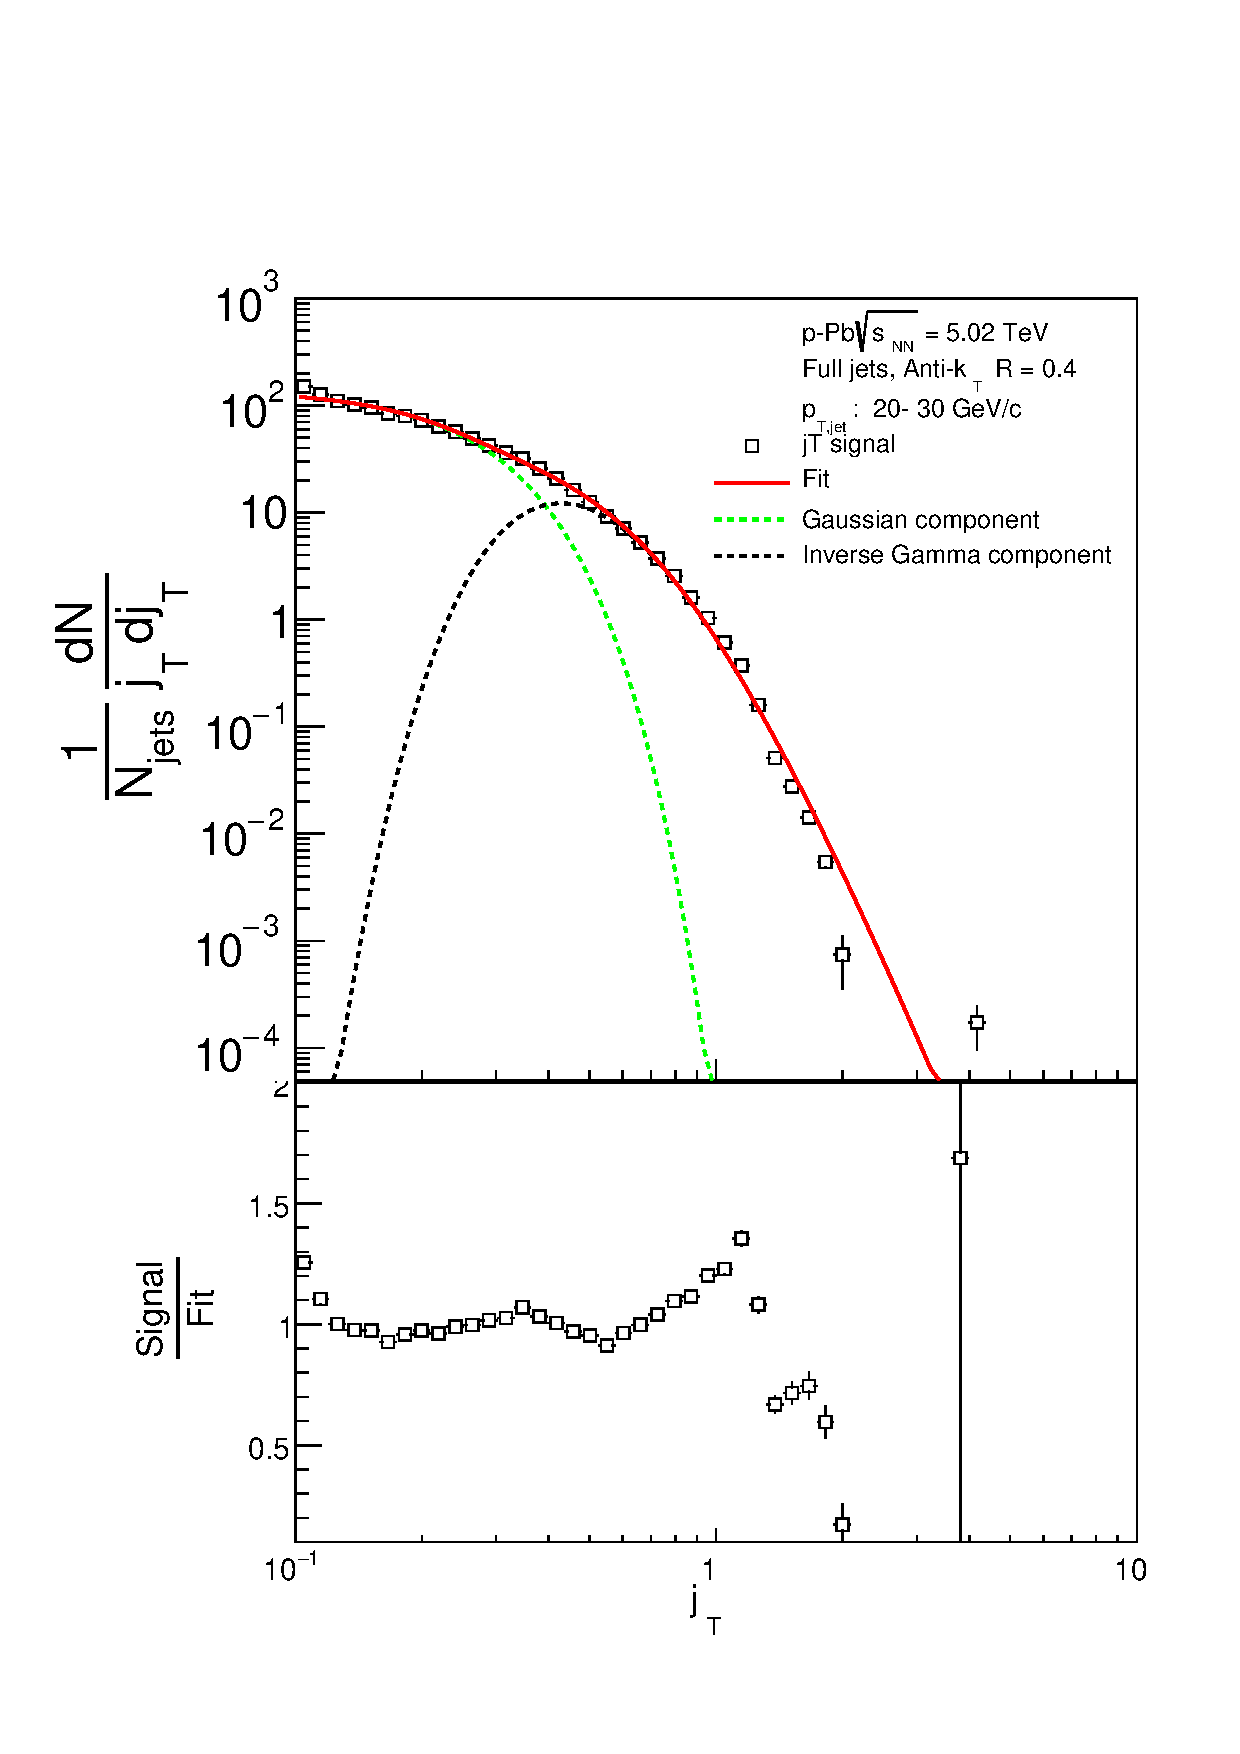
\includegraphics[width=0.95\textwidth]{RooUnfold/figs/JetConejTSignalFit/JetConejTSignalFitNFin00JetPt02perconeBgBayes}
%\end{subfigure}
%\begin{subfigure}{0.24\textwidth}
%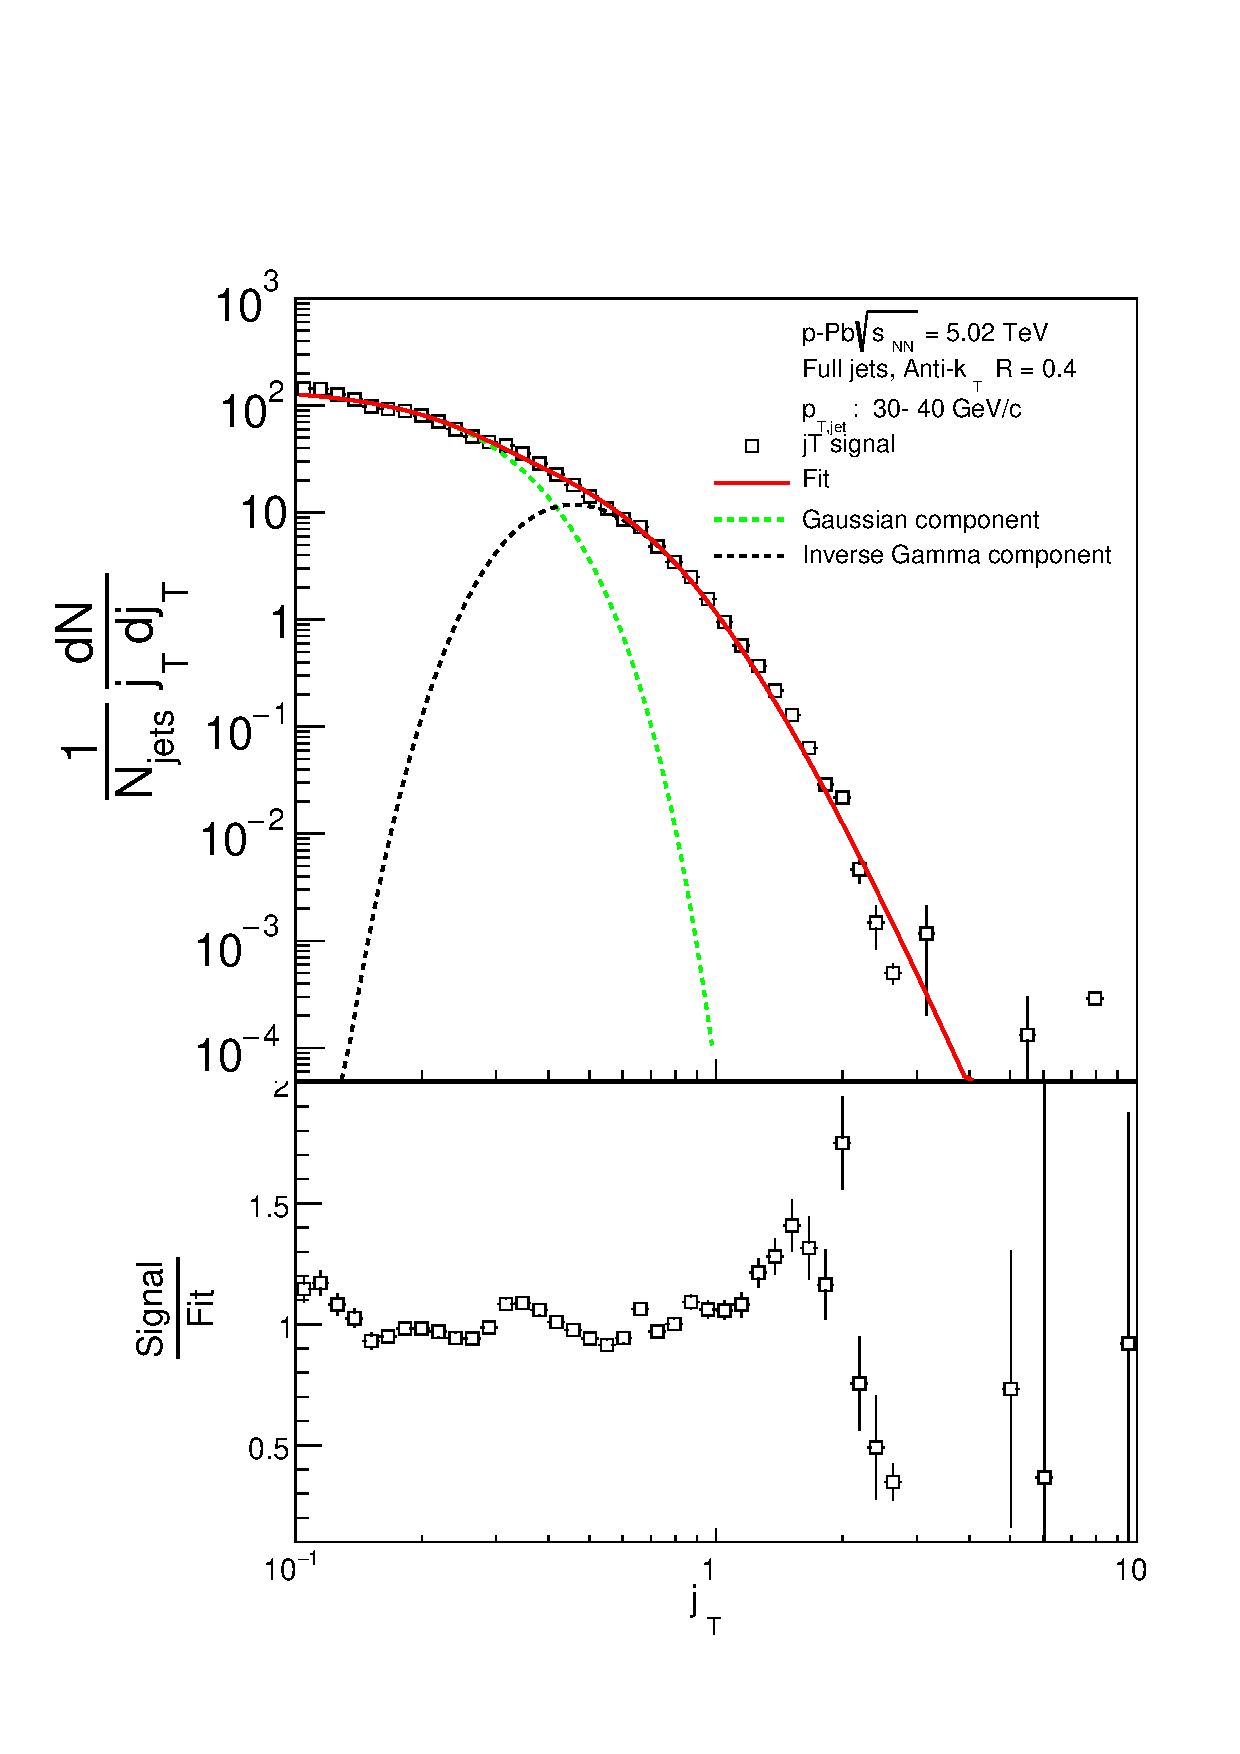
\includegraphics[width=0.95\textwidth]{RooUnfold/figs/JetConejTSignalFit/JetConejTSignalFitNFin00JetPt03perconeBgBayes}
%\end{subfigure}
\begin{subfigure}{0.24\textwidth}
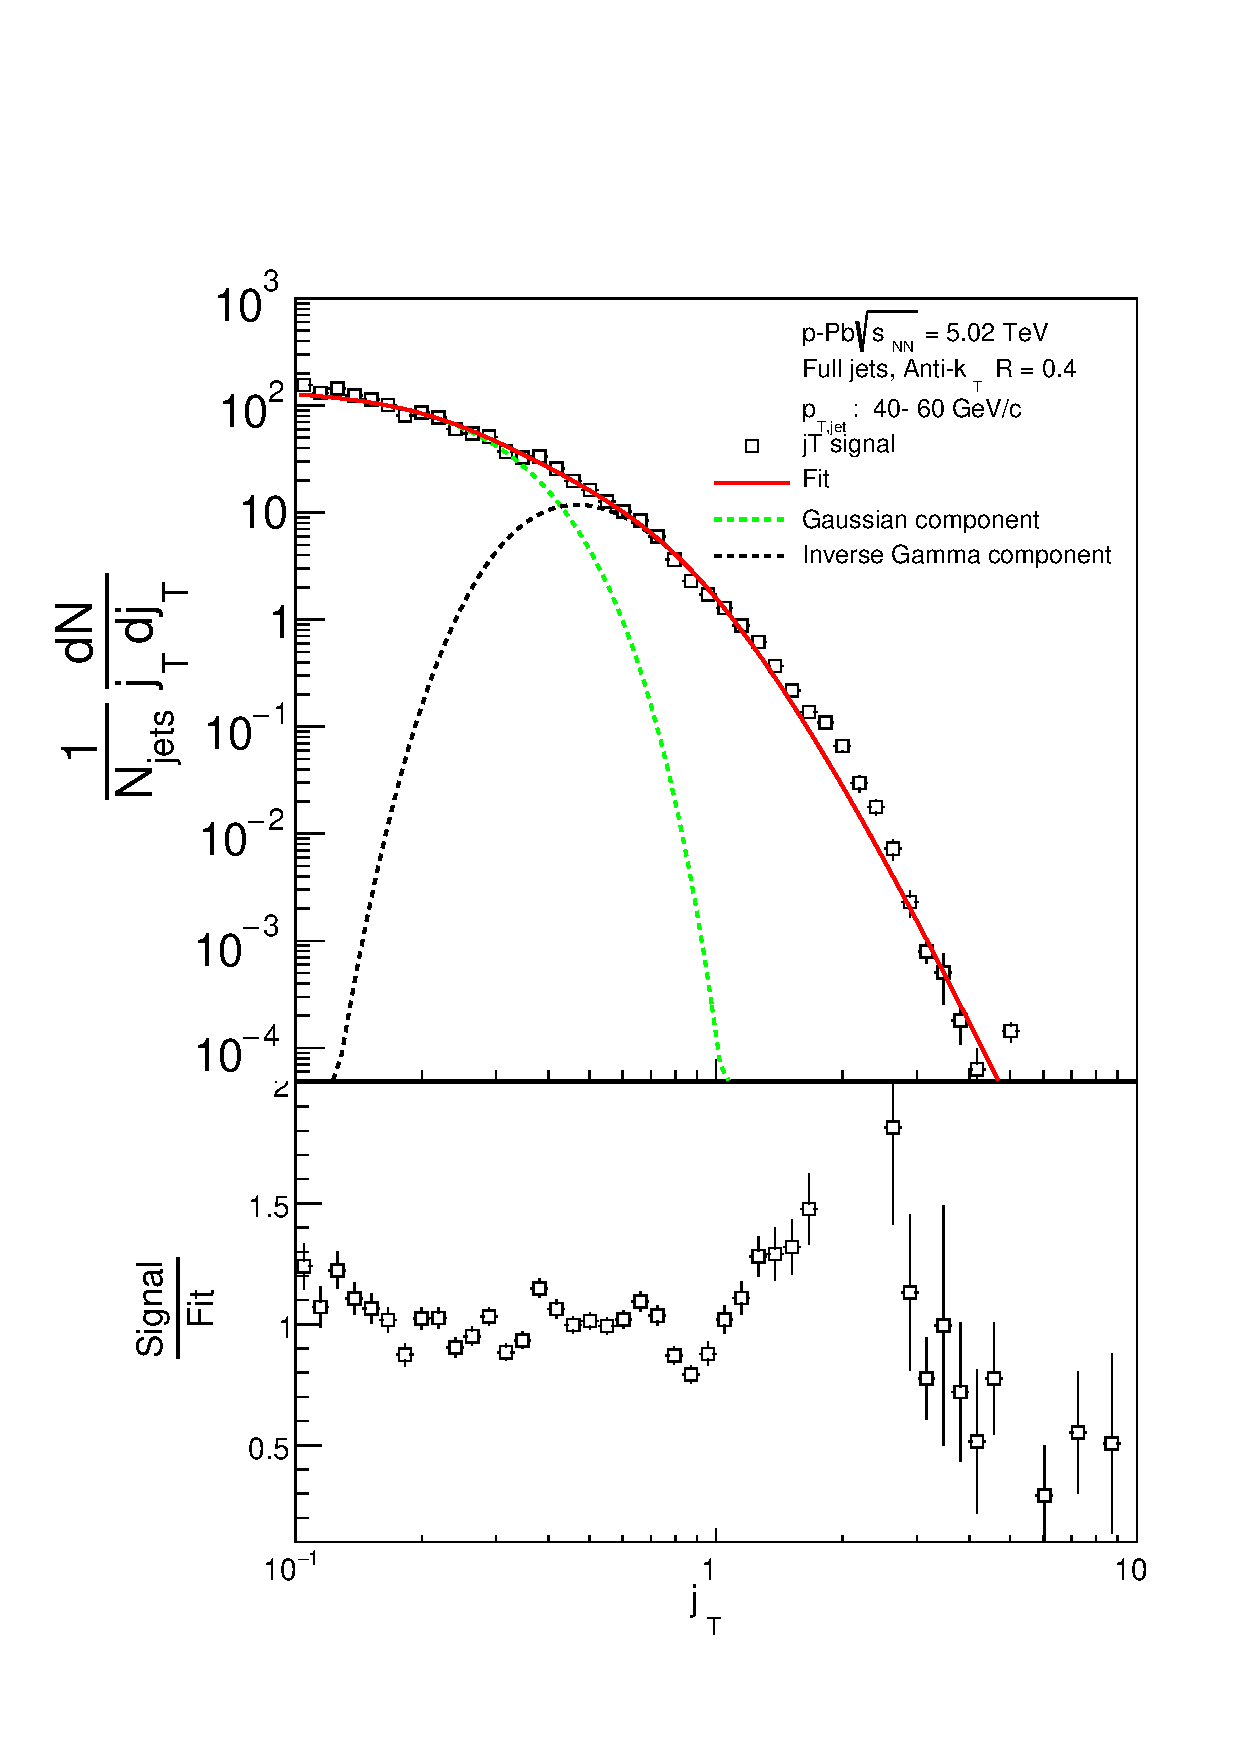
\includegraphics[width=0.95\textwidth]{results/JetConejTSignalFit/JetConejTSignalFitNFin00JetPt04perconeBgBayes}
\end{subfigure}
\begin{subfigure}{0.24\textwidth}
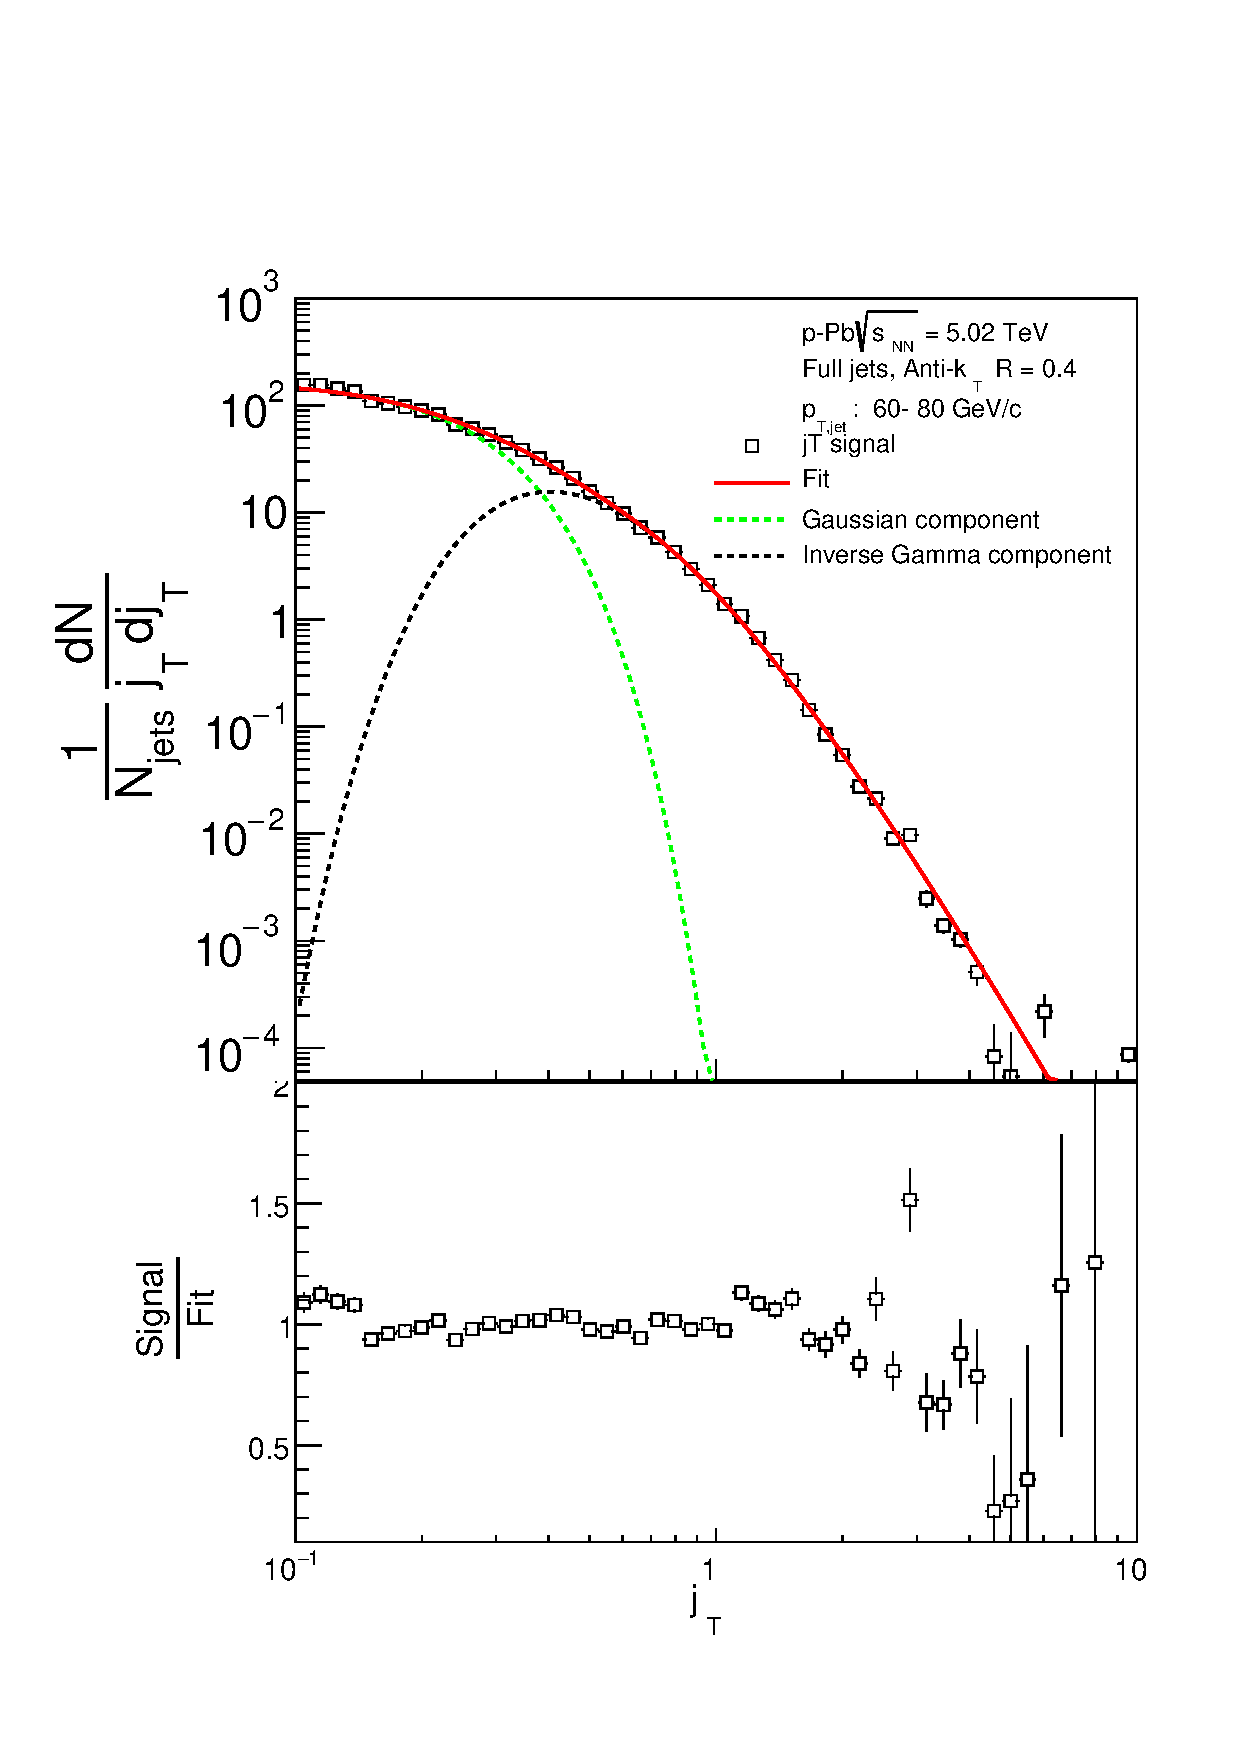
\includegraphics[width=0.95\textwidth]{results/JetConejTSignalFit/JetConejTSignalFitNFin00JetPt05perconeBgBayes}
\end{subfigure}
\begin{subfigure}{0.24\textwidth}
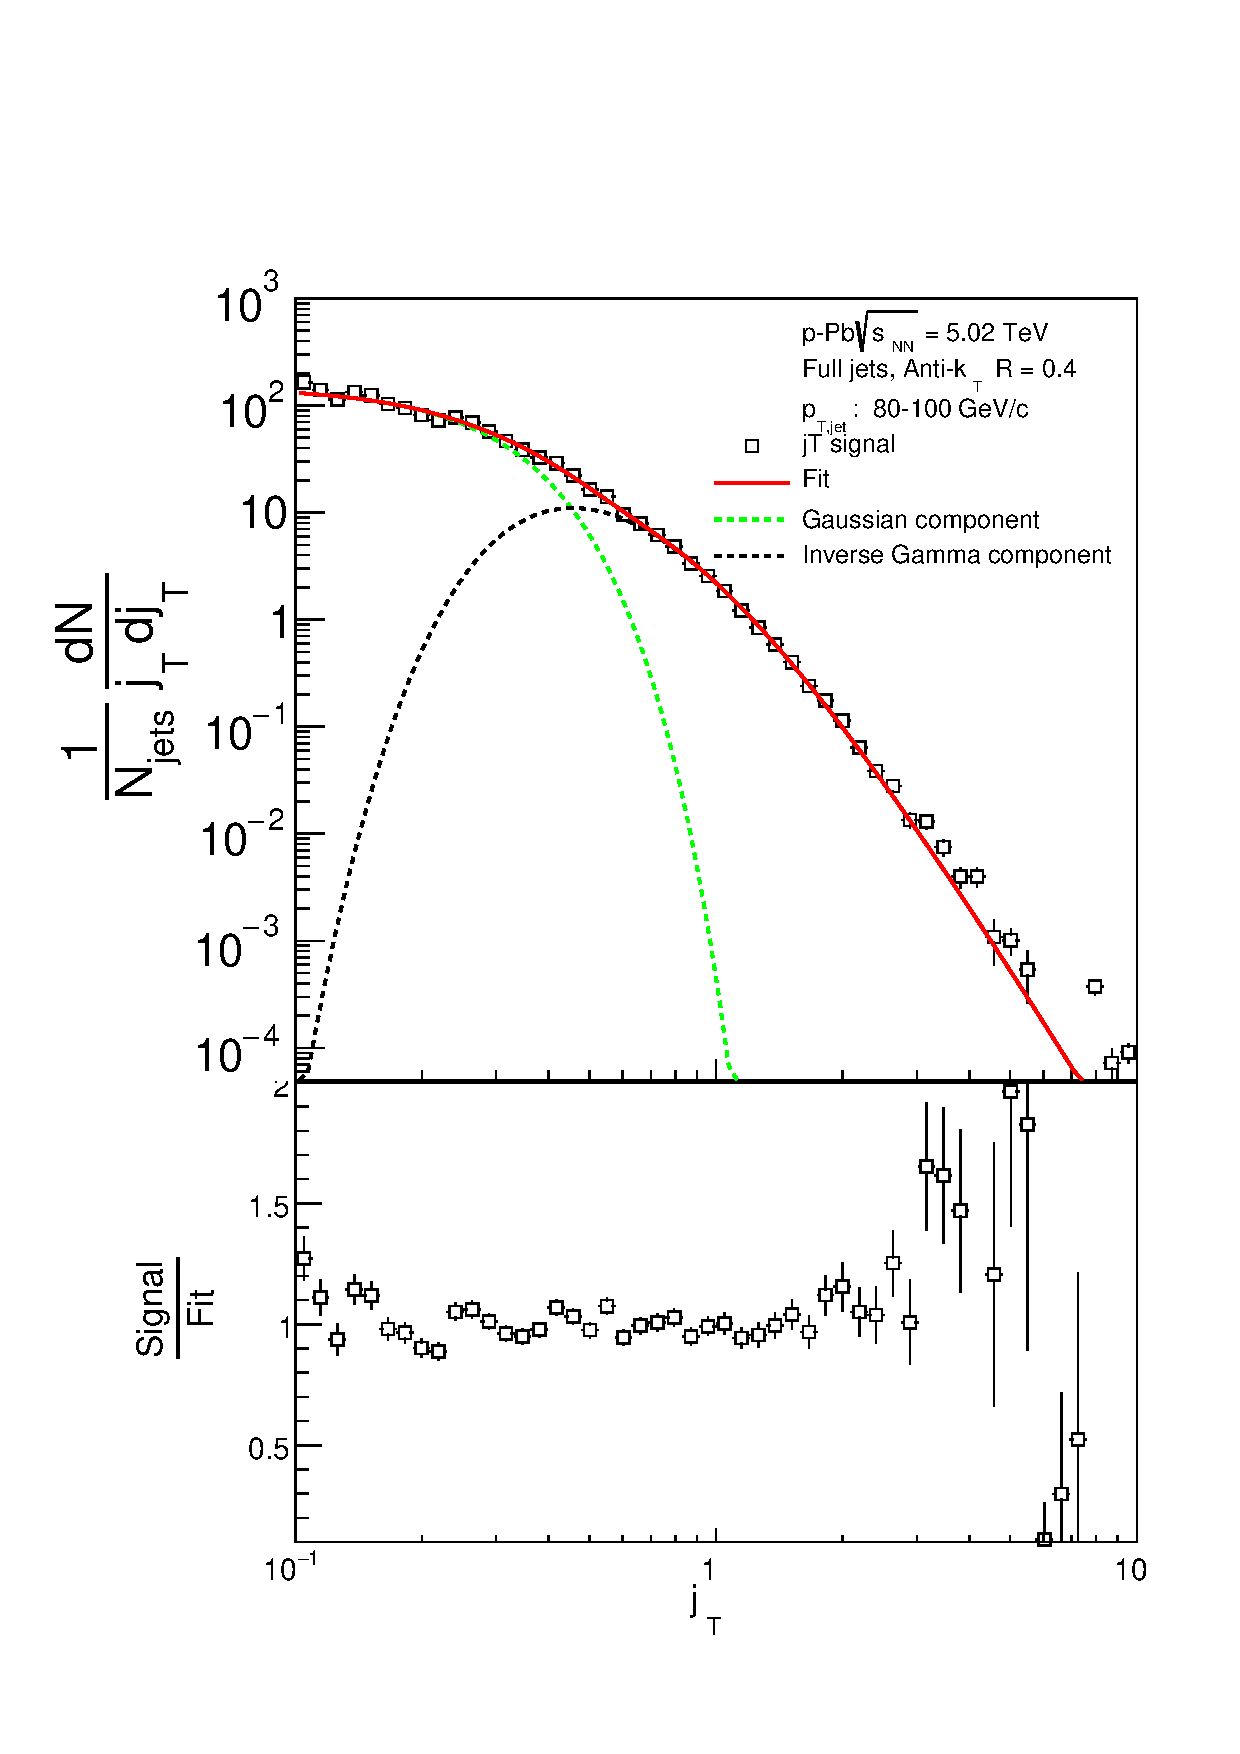
\includegraphics[width=0.95\textwidth]{results/JetConejTSignalFit/JetConejTSignalFitNFin00JetPt06perconeBgBayes}
\end{subfigure}
\begin{subfigure}{0.24\textwidth}
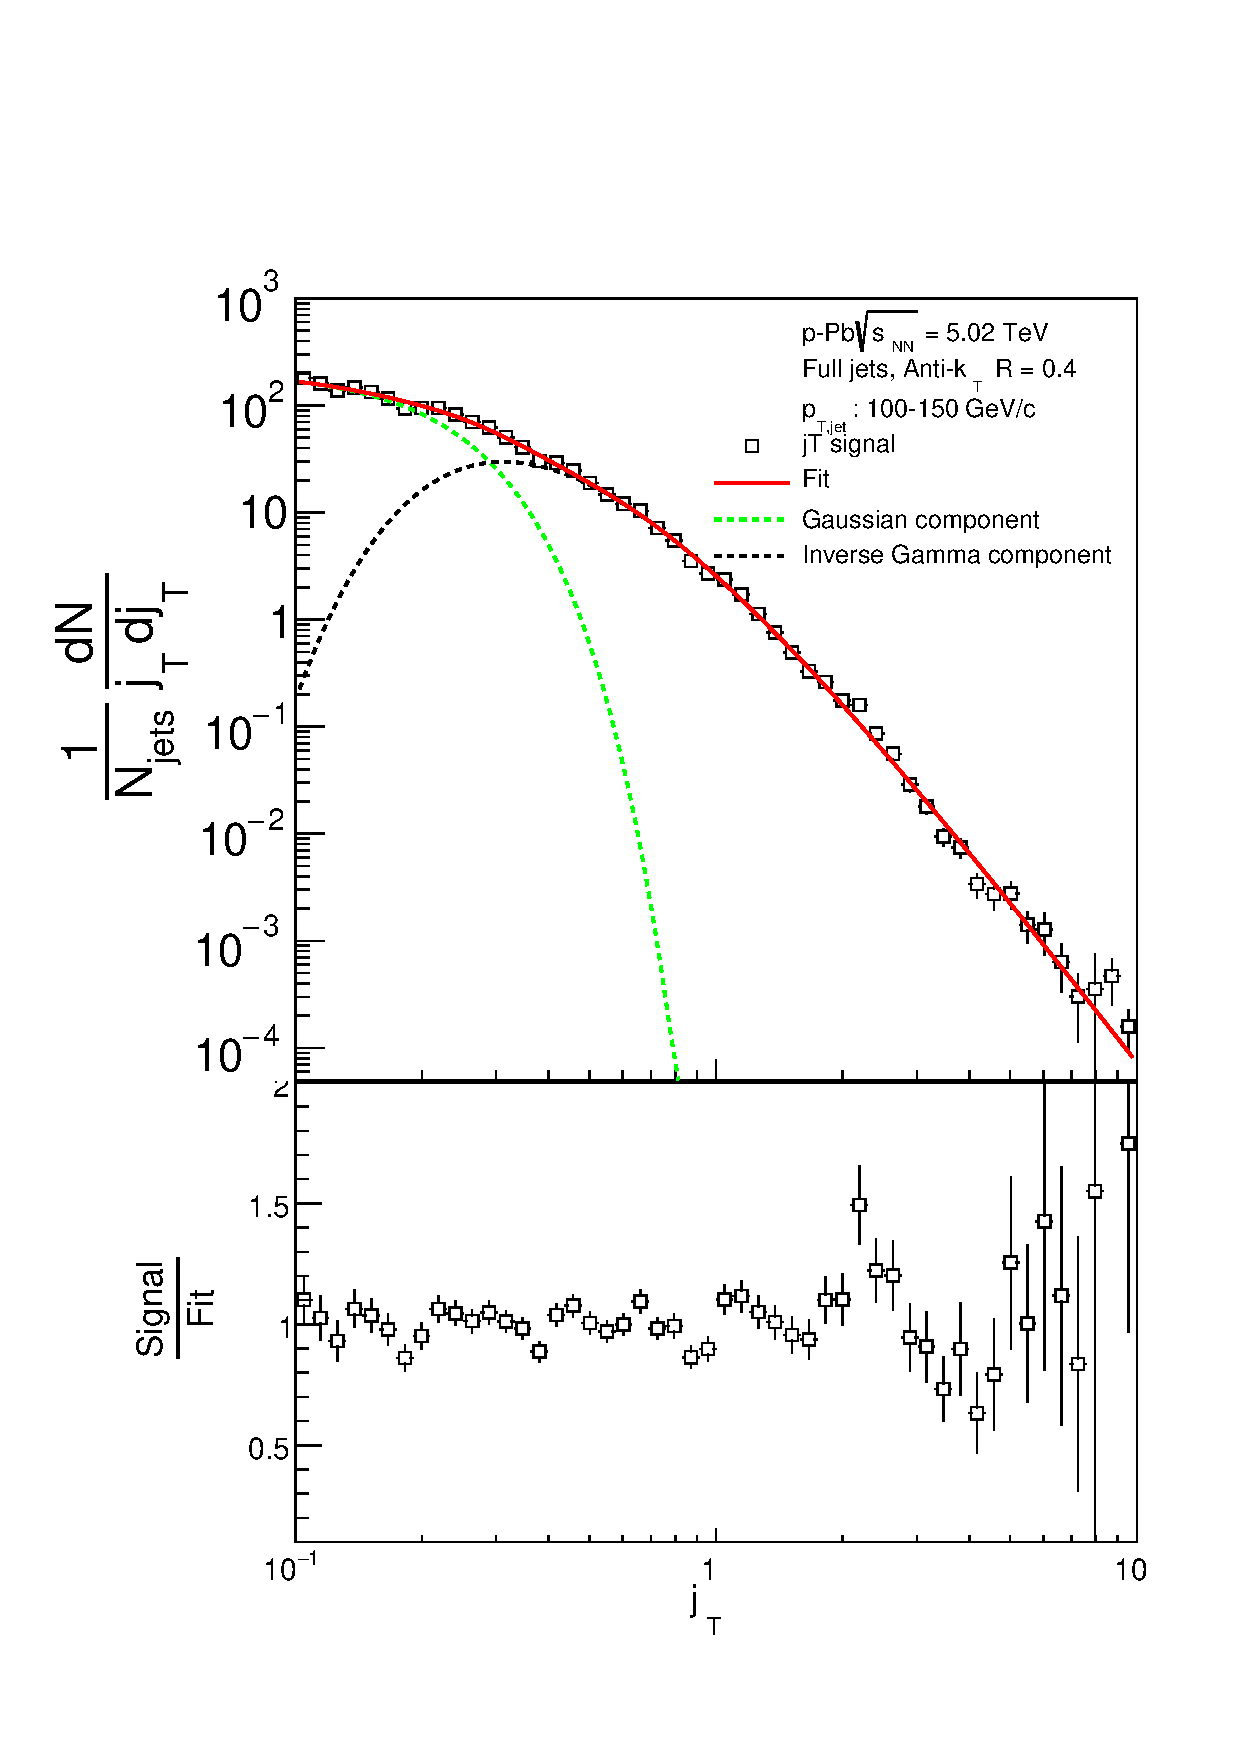
\includegraphics[width=0.95\textwidth]{results/JetConejTSignalFit/JetConejTSignalFitNFin00JetPt07perconeBgBayes}
\end{subfigure}
\caption{$j_T$ signal fits in different jet $p_T$ bins}
\label{fig:fits}
\end{figure}




\subsubsection{Results}
RMS and yield results with systematic errors are shown separately in figure \ref{fig:rmsyield}. Figure \ref{fig:rms} shows RMS values for both components combined. The figure also includes results from a PYTHIA simulation. 
\begin{figure}[htb]
\begin{subfigure}{0.5\textwidth}
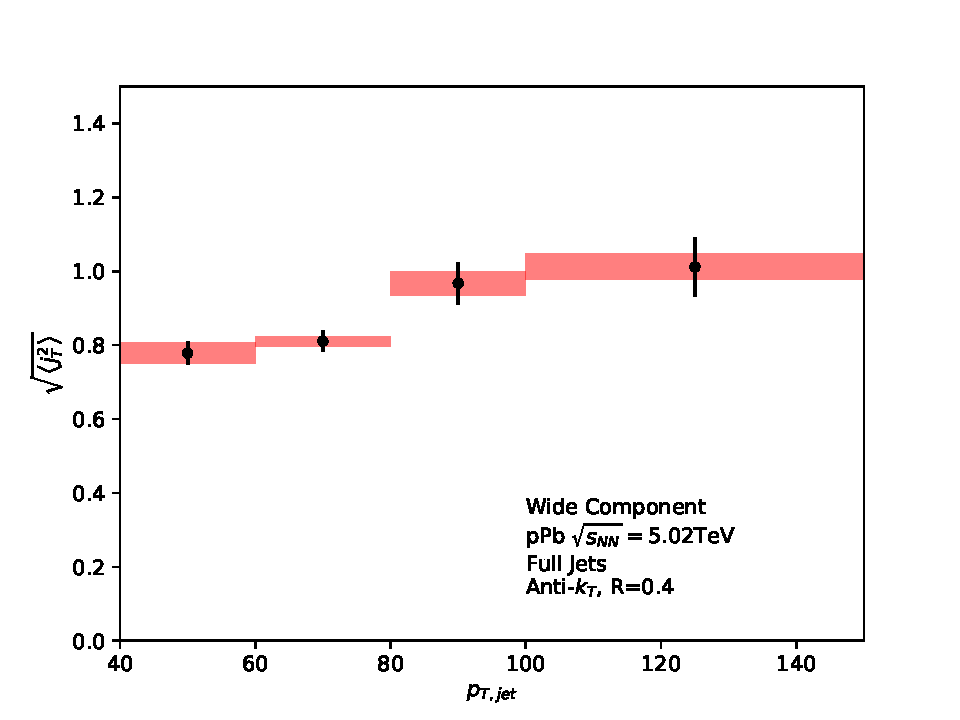
\includegraphics[width=0.95\textwidth]{results/gammaRMSWithSystematics}
\end{subfigure}
%\begin{subfigure}{0.5\textwidth}
%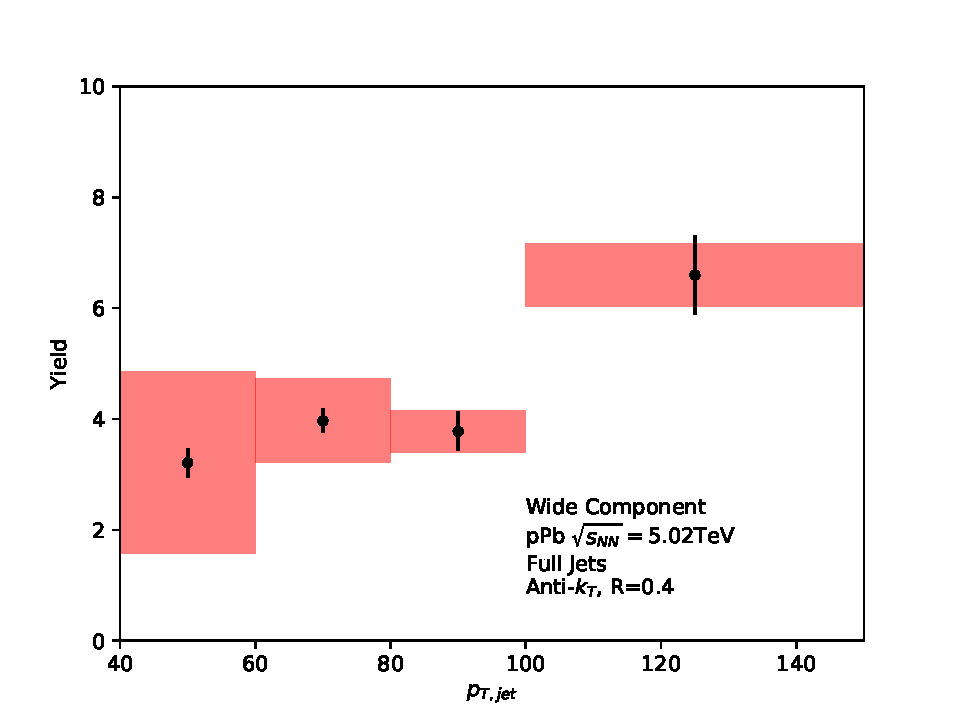
\includegraphics[width=0.95\textwidth]{results/gammaYieldWithSystematics}
%\end{subfigure}
\begin{subfigure}{0.5\textwidth}
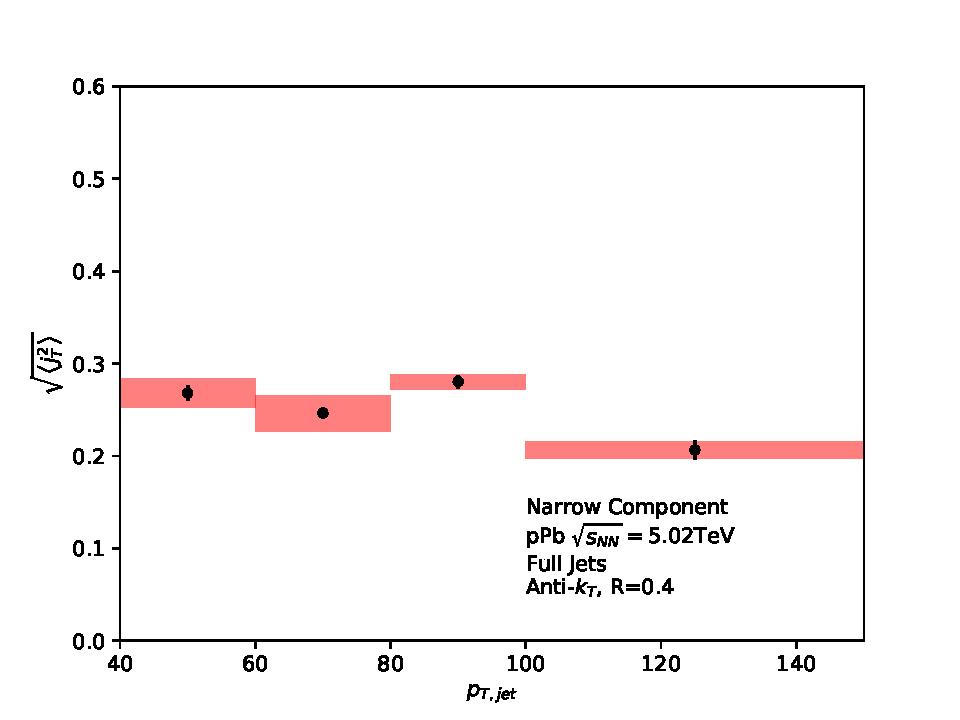
\includegraphics[width=0.95\textwidth]{results/gausRMSWithSystematics}
\end{subfigure}
%\begin{subfigure}{0.5\textwidth}
%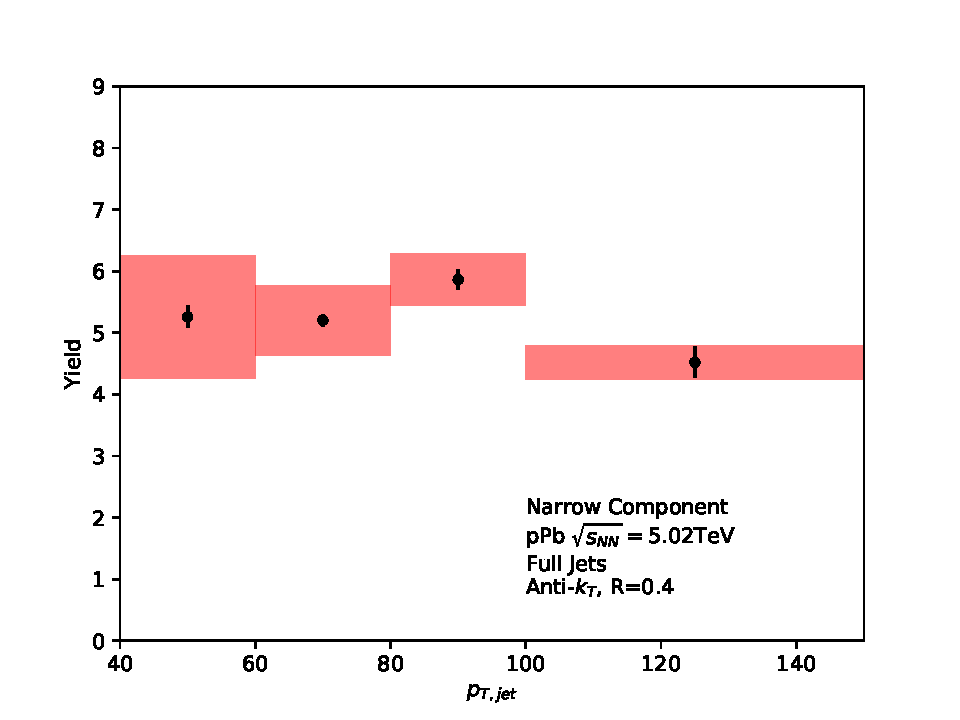
\includegraphics[width=0.95\textwidth]{results/gausYieldWithSystematics}
%\end{subfigure}
\caption{RMS values extracted from the fits for the gaussian (narrow) and inverse gamma (wide) components}
\label{fig:rmsyield}
\end{figure}

\begin{figure}[htb]
\begin{subfigure}{0.5\textwidth}
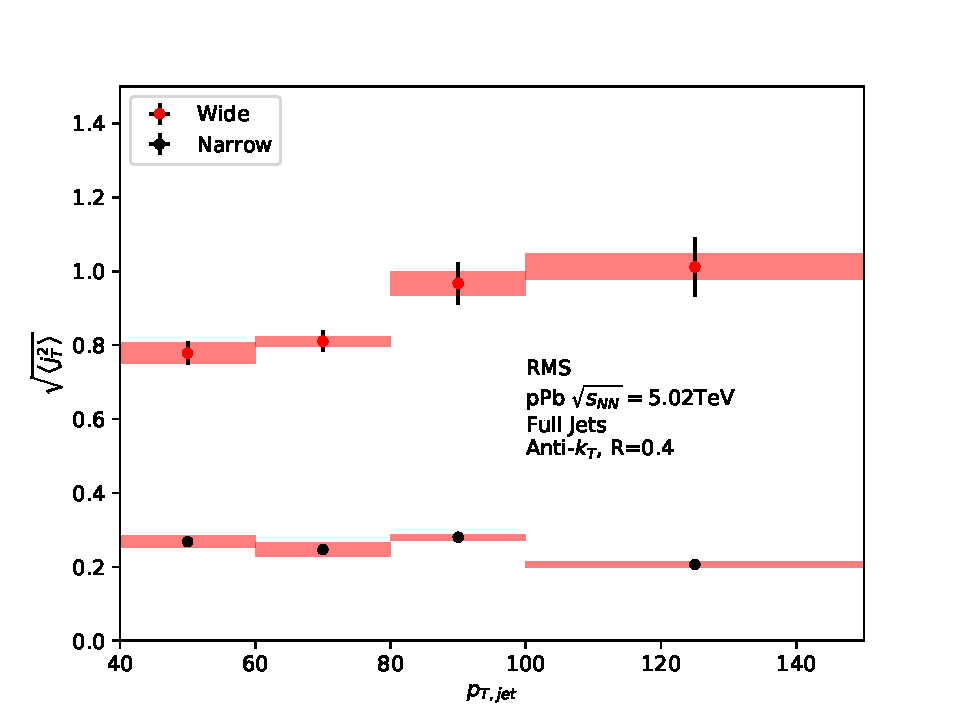
\includegraphics[width=0.95\textwidth]{results/RMSWithSystematics}
\end{subfigure}
\begin{subfigure}{0.5\textwidth}
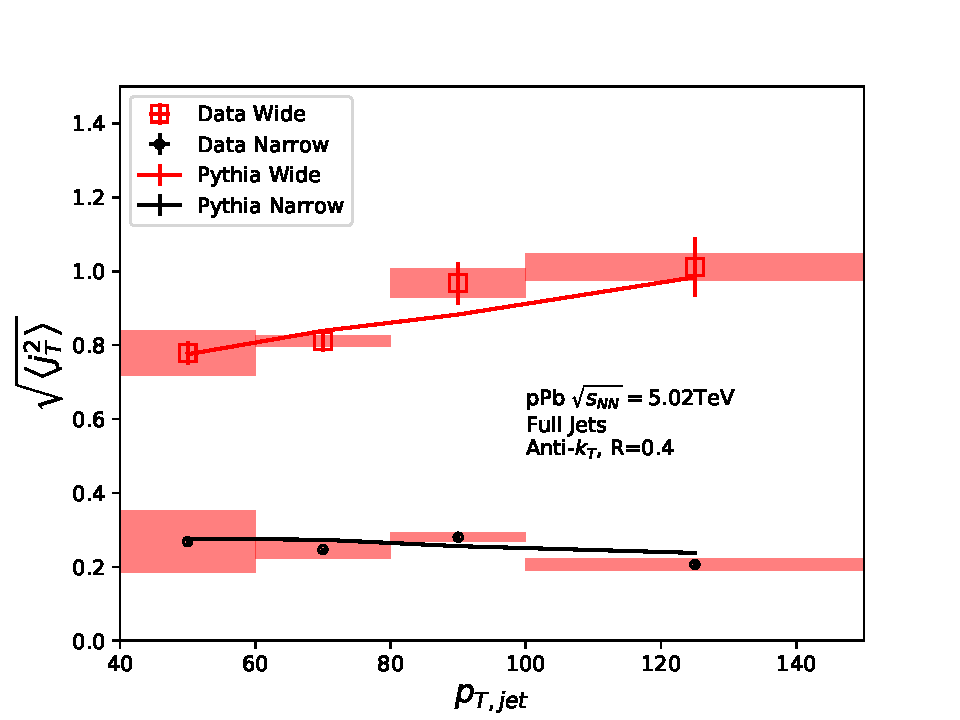
\includegraphics[width=0.95\textwidth]{results/RMSWithSystematics_Pythia}
\end{subfigure}
\caption{RMS values extracted from the fits for the gaussian (narrow) and inverse gamma (wide) components}
\label{fig:rms}
\end{figure}

\subsection{Comparison to dihadron results}
Comparison to RMS values in dihadron analysis~\cite{jussi} are shown in figure \ Dihadron results from~\cite{jussi}. For comparison the dihadron trigger $p_T$ bins are converted to jet $p_T$ bins and vice versa. Bin-by-bin comparison is still not possible, but dihadron analysis gives systematically larger RMS values. This could be caused by several kinematical factors. In jet $j_T$ analysis the jet cone limits possible $j_T$ values and thus the width and RMS of the $j_T$ distributions. The effect of this limitation can be studied by changing the cone size as is described in section \ref{sec:Rstudy}. 

Comparison to $j_T$ results from dihadron analysis ~\cite{jussi} is shown in figure \ref{fig:DihadronComparison}. Trigger $p_T$ bins used in dihadron analysis are converted to jet $p_T$ bins using observed average jet $p_T$ values in leading track momentum bins. Simlarly jet $p_T$ bins are converted to $p_{T,\mathrm{trigger}}$ bins using average leading track $p_T$ values in $p_{T,\mathrm{jet}}$ bins.

The trends are similar in dihadron and jet $j_T$ results. Wide component RMS values tend to increase with increasing $p_{T,\mathrm{trigger}}$/$p_{T,\mathrm{jet}}$. Narrow component RMS increases slightly in dihadron analysis but not in jet $j_T$, WHY? (Depends on $x_{||}$ bin in dihadron)

In general dihadron $j_T$ gives wider distributions with larger RMS values. In jet analysis the cone size limits width and thus the RMS values. The effect of this limitation can be studied by changing the cone size as is described in section \ref{sec:Rstudy}.

Additionally the leading track is an imperfect estimate of the jet/original parton. Because the leading track in general is at an angle compared to the jet axis, the resulting $j_T$ values are different. In practice the jet axis found by the jet finding algrorithm tends to minimize the average $j_T$ of jet constituents. Thus the yield at high $j_T$ is limited and the RMS values are smaller.


\begin{figure}[htb]
\begin{subfigure}{0.5\textwidth}
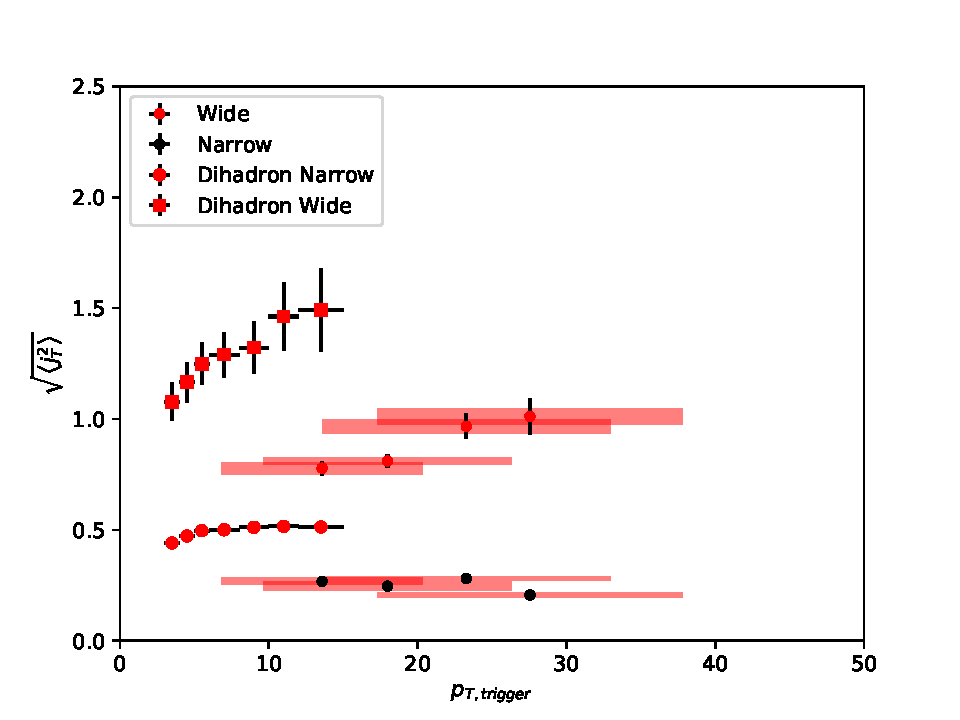
\includegraphics[width=0.99\textwidth]{/Users/tuomas/OneDrive/work/032.JTAnalysis/Unfolding/RooUnfold/PythonFigures/RMSWithSystematics_DihadronTriggerPt.pdf}
\end{subfigure}
\begin{subfigure}{0.5\textwidth}
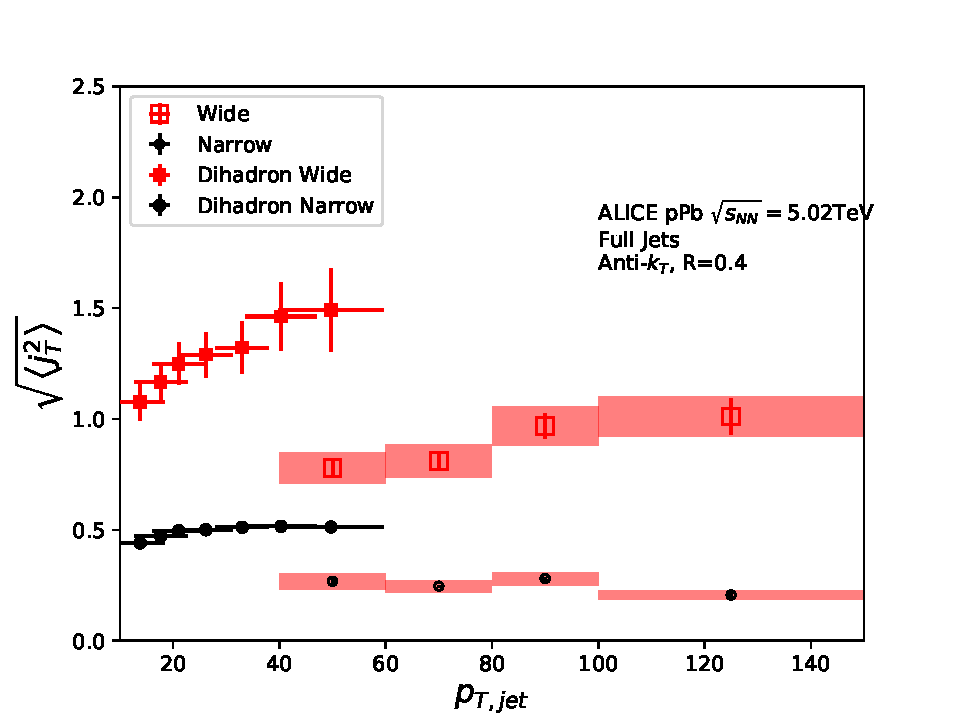
\includegraphics[width=0.99\textwidth]{/Users/tuomas/OneDrive/work/032.JTAnalysis/Unfolding/RooUnfold/PythonFigures/RMSWithSystematics_DihadronJetPt.pdf}
\end{subfigure}
\caption{Jet $j_T$ results are compared to results obtained in the dihadron analysis. This is done both in jet $p_T$ and trigger $p_T$ bins by converting between them.}
\label{fig:dihadroncomparison}
\end{figure}

\subsection{Different $R$ parameters}
\label{sec:Rstudy}
Study the effect of cone sizes on $j_T$ distribution in particle level Pythia.

Increasing the cone size of jets gives more room for high $j_T$ tracks. This is seen in the individual $j_T$ distributions as increased high $j_t$ production. At low $j_T$ there is no change.

When looking at RMS values from wide component we see an increase/decrease of about 10\% when going from $R=0.4$ to $R=0.5$/$R=0.3$.

The message from narrow component RMS values is less clear. At low jet $p_T$ the behaviour is similar, but at high $p_T$ the order is reversed. 
\begin{figure}[htp]
\centering
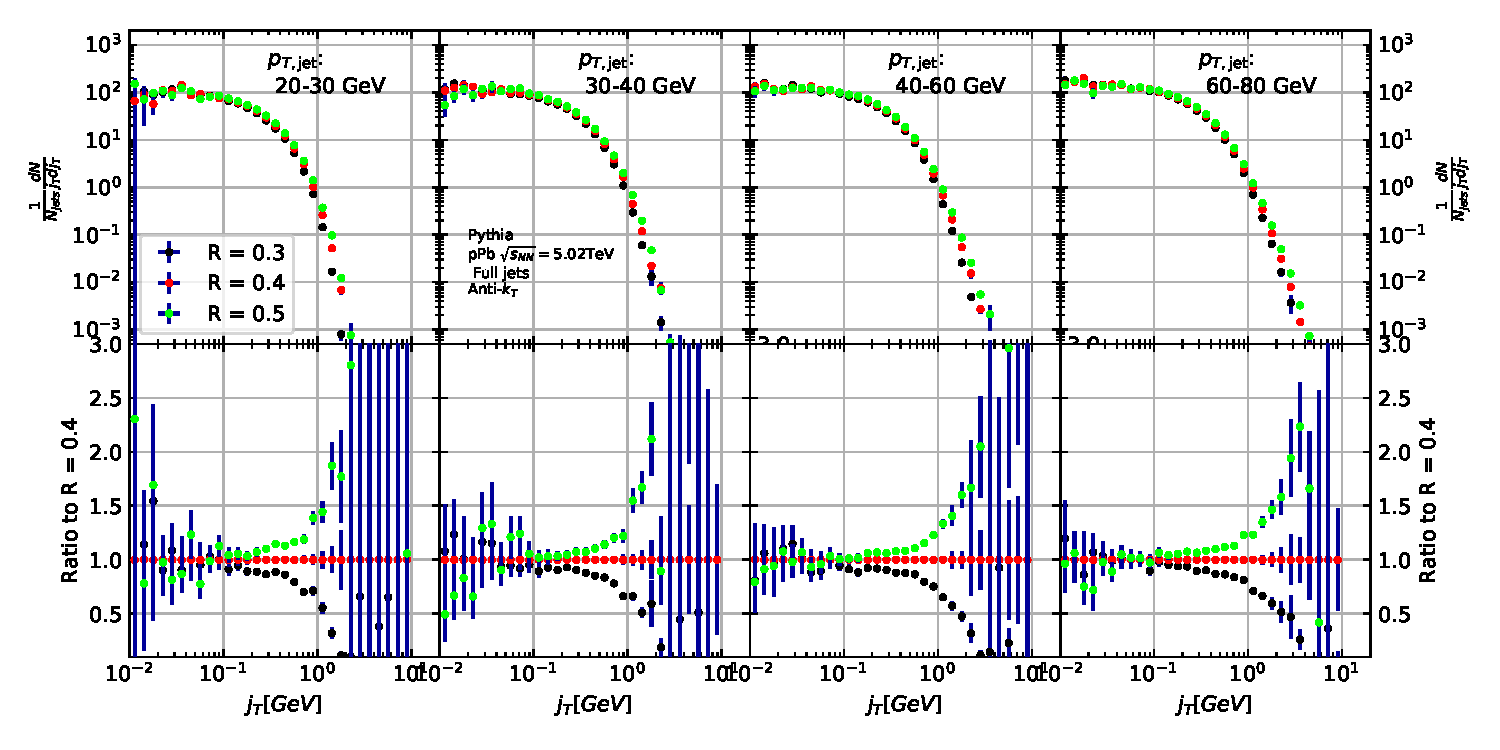
\includegraphics[width=0.6\textwidth]{results/RcomparisonSignal.pdf}
\caption[Pythia $R$ parameters $j_T$]{Effect of changing $R$ parameter in jet finding on $j_T$ distributions}
\label{fig:RcomparisonjT}
\end{figure}


\begin{figure}[htp]
\centering
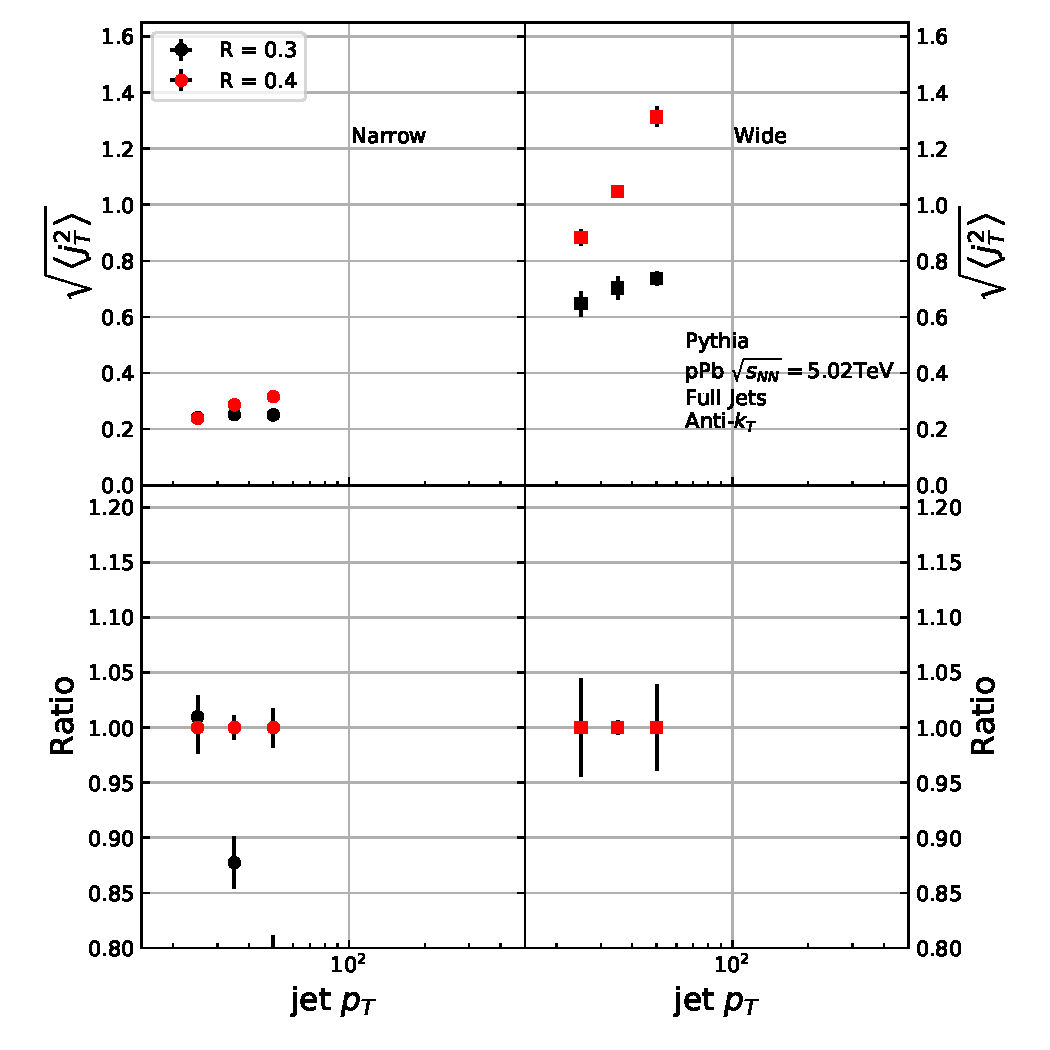
\includegraphics[width=0.6\textwidth]{/Users/tuomas/OneDrive/work/037.JtPaper/jet-jt-paper-cern-preview/figures/results/RcomparisonRMS.pdf} \\
\caption[Pythia $R$ parameters RMS]{Effect of changing $R$ parameter in jet finding on narrow and wide component RMS values. Wide component RMS values increase with increasing cone size.}
\label{fig:RcomparisonRMS}
\end{figure}